\documentclass[lettersize,journal]{IEEEtran}
\usepackage{amsmath,amsfonts}
\usepackage{algorithmic}
\usepackage{algorithm}
\usepackage{array}
\usepackage[caption=false,font=normalsize,labelfont=sf,textfont=sf]{subfig}
\usepackage{textcomp}
\usepackage{stfloats}
\usepackage{url}
\usepackage{verbatim}
\usepackage{graphicx}
\usepackage{capt-of}
%\usepackage{cite}
\usepackage[backend=biber,style=ieee]{biblatex}
\addbibresource{refs.bib}
\hyphenation{op-tical net-works semi-conduc-tor IEEE-Xplore}
% updated with editorial comments 8/9/2021

\begin{document}

\title{A no reference pointcloud quality assessment with neural network}

\author{\IEEEmembership{Mathias Aagaard, Magnus Karlsen}}
        % <-this % stops a space


% The paper headers
%\markboth{Journal of \LaTeX\ Class Files,~Vol.~14, No.~8, August~2021}%
%{Shell \MakeLowercase{\textit{et al.}}: A Sample Article Using IEEEtran.cls for IEEE Journals}

\maketitle

\begin{abstract}

\end{abstract}

\begin{IEEEkeywords}
Pointcloud, quality, Neural network
\end{IEEEkeywords}

\section{Introduction}
Point clouds serve as a foundational data structure in robotic 3D scanning, enabling accurate geometric reconstruction of objects and environments. The quality of these point clouds is critical for downstream tasks such as object modeling, inspection, localization, and navigation. A reliable metric for local point cloud quality assessment (PCQA) is therefore indispensable, especially in automated systems that must decide whether a re-scan is warranted in real-time. Existing methods often rely on global point density or volume-based metrics which are computationally efficient but poorly reflect surface-level fidelity.

This report proposes a novel, data-driven approach for estimating local surface density — a more faithful representation of point cloud quality — using neural networks. While surface density has been recognized as superior to volume density for capturing local structure, its direct computation is computationally expensive and infeasible for real-time or large-scale scanning applications. The proposed method overcomes this limitation by learning to infer surface density from a set of rapidly computable features that include both local volume density and geometric bias descriptors.

To ground this concept, a 2D analogy is presented where the limitations of area-based density measures in capturing edge fidelity are illustrated. This motivates the extension of the concept to 3D, where volume density — analogous to area density in 2D — serves as a rough but computable approximation of true surface fidelity. The core idea of this methodology is to leverage this correlation and predict surface density indirectly by using a neural network trained on volume-based features augmented with geometry-aware descriptors.

The ultimate goal is to produce a real-time capable PCQA mechanism that retains high sensitivity to quality-relevant features such as surface curvature, holes, and geometric distortions — enabling smarter, self-optimizing robotic scanning systems.

<\section{Related Works}

\section{Methodology}
\subsection{Features Used in Neural Network}
\label{sec:features}
The features can be devided into two groups, volume density and geometry bias. Volume density captures the local point concentration around a given point, whereas geometry bias accounts for how local surface geometry may distort this measure.

\subsection*{Volume Density Features}
Local volume density can be estimated using either a fixed-radius approach, which counts the number of neighbors within a constant radius for all points, or a fixed-number-of-neighbors approach, which measures the radius required to enclose a fixed number of neighbors around each point. The fixed-radius approach allows the volume density feature to capture information about holes and gaps in the poincloud. In contrast, the fixed-number-of-neighbors approach may obscure such features, as the nearest-neighbor algorithms tend to sample around or beyond holes, reducing their impact on the density estimate (see Figure~\ref{fig:radVSnbh_VD}). 
To ensure high sensitivity to holes, the fixed-radius approach is preferred. However, a fixed radius is unsuitable across varying point clouds, as it can yield inconsistent neighborhood sizes. 

Instead, an adaptive radius is defined as the average radius from the fixed-number-of-neighbors approach, based on 20 neighbors as shown in Algorithm \ref{alg:volume_density}. 
\begin{algorithm}[H]
\caption{Compute Volume Density Features}
\label{alg:volume_density}
\begin{algorithmic}[1]
\STATE \textbf{Input:} Point cloud $P$
\STATE Initialize list of radii $R \leftarrow []$
\FOR{each point $p \in P$}
  \STATE Find 20 nearest neighbors of $p$
  \STATE Compute radius $r_p$ containing these 20 neighbors
  \STATE Append $r_p$ to $R$
\ENDFOR
\STATE Compute average radius $\bar{r} \leftarrow \text{mean}(R)$
\FOR{each point $p \in P$}
  \STATE Count the number of neighbors within $\bar{r}$ (Euclidean ball)
  \STATE Save this count as $n_p$
\ENDFOR
\STATE \textbf{Output:} Average radius $\bar{r}$ and list $\{n_p\}$ of points inside Euclidean ball.
\end{algorithmic}
\end{algorithm}



The average radius is used and included as an explicit input feature. This enables the network to interpret local volume density consistently across different scales and sampling resolutions.
The volume density then consists of two features:
\begin{itemize}
    \item \textbf{Average radius}, equal for all points in a single pointcloud 
    \item \textbf{Points inside average radius}, varies for every point
\end{itemize}

\begin{figure}[H]
    \centering
    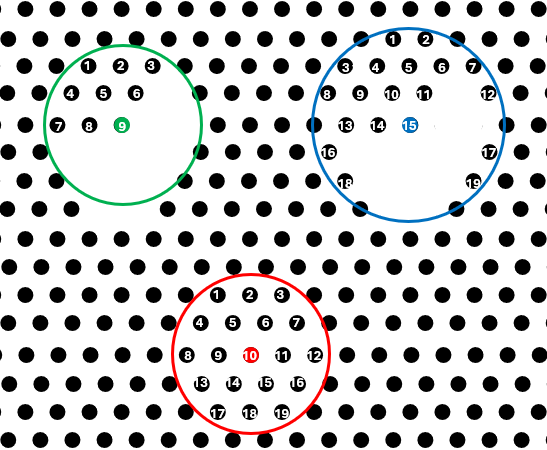
\includegraphics[width=0.4\textwidth]{figures/RadiusVSPoint_based.png}
    \caption{Comparison of volume density estimation using fixed-radius versus fixed-neighborhood methods in the presence of holes.\textbf{Red:} Uniform point distribution with no missing data; both methods yield consistent estimates.\textbf{Green:} Fixed-radius approach near a hole; the radius remains unchanged, but significantly fewer neighbors are included, revealing the presence of a gap.\textbf{Blue:} Fixed-number-of-points approach near a hole; the radius increases slightly to maintain the neighbor count, sampling around the hole reduces sensitivity to the lack of points.}\label{fig:radVSnbh_VD}
\end{figure}

\subsection*{Geometry Bias Features}
Just as a straight line represents the shortest distance between two points, a planar surface is the minimal-area surface that connects any three points. Consequently, a planar region will generally exhibit lower volume density than a curved surface with the same surface density. However, not all geometric influences on volume density are easily measurable. To account for this, multiple geometric features are incorporated to enable the neural network to learn the underlying patterns that define the local geometry bias.
For simplicity, geometry features are computed using the k-nearest neighbors algorithm with a neighborhood size of 20. While this differs slightly from the method used for volume density, the use of the same neighborhood size as the average radius minimizes discrepancies between the feature sets. Five eigenvalue-based features and one gradient-based feature were initially selected to represent the geometry bias. 

The eigenvalue-based features and their formulations are shown in Equation~\ref{eq:eigenvalue_features}, computed using the \texttt{pyntcloud} library. 

\begin{equation}
\begin{aligned}
    &\lambda_1 \geq \lambda_2 \geq \lambda_3 \geq 0 \\
    \textbf{Curvature} &= \frac{\lambda_3}{\lambda_1 + \lambda_2 + \lambda_3} \\
    \textbf{Linearity} &= \frac{\lambda_1 - \lambda_2}{\lambda_1} \\
    \textbf{Planarity} &= \frac{\lambda_2 - \lambda_3}{\lambda_1} \\
    \textbf{Omnivariance} &= {\lambda_1 + \lambda_2 + \lambda_3}^{1/3} \\
    \textbf{Eigensum} &= \lambda_1 + \lambda_2 + \lambda_3
\end{aligned}
\label{eq:eigenvalue_features}
\end{equation}

where $\lambda_1$, $\lambda_2$ and $\lambda_3$ are the 3 eigenvalues of the covariance matrix for each neighborhood.

For the gradient-based feature, the mean gradient difference was used to quantify local surface variation within a neighborhood. Gradients were computed using the weighted least squares surface fitting approach implemented in the pcdiff library [REF]. Each local surface was fitted to the quadratic form seen in Equation~\ref{eq:surface_fit}:

\begin{equation}
f(x, y) = c_0 + c_1 x + c_2 y + c_3 x^2 + c_4 x y + c_5 y^2
\label{eq:surface_fit}
\end{equation}

The gradient at each point in the neighborhood was then derived analytically with Equation~\ref{eq:grad_vector}.

\begin{equation}
\nabla f(x, y) =
\begin{bmatrix}
\frac{\partial f}{\partial x} \\
\frac{\partial f}{\partial y}
\end{bmatrix}
=
\begin{bmatrix}
c_1 + 2c_3 x + c_4 y \\
c_2 + 2c_5 y + c_4 x
\end{bmatrix}
\label{eq:grad_vector}
\end{equation}

To compute the gradient difference, the L2 norm was applied to the difference between the center points gradient and that of each of its neighbors. The mean of these differences across the neighborhood was used as the final gradient-based feature.

The outputs, for all geometry features, are plotted in Figure~\ref{fig:feature_plot}, for a neighborhood size of 20 points. Omnivariance appears to provide the most substantial information about local geometry. However, both omnivariance and eigensum are proportional to the eigenvalues of the covariance matrix, which scale with the square of the local mesh size. As a result, these features outperformed volume density features during training, but lacked sensitivity to holes and gaps in the data. This led to a model which failed to detect simple voids in the point cloud. Consequently, omnivariance and eigensum were excluded from the final feature set.

\begin{figure*}[h]
    \centering
    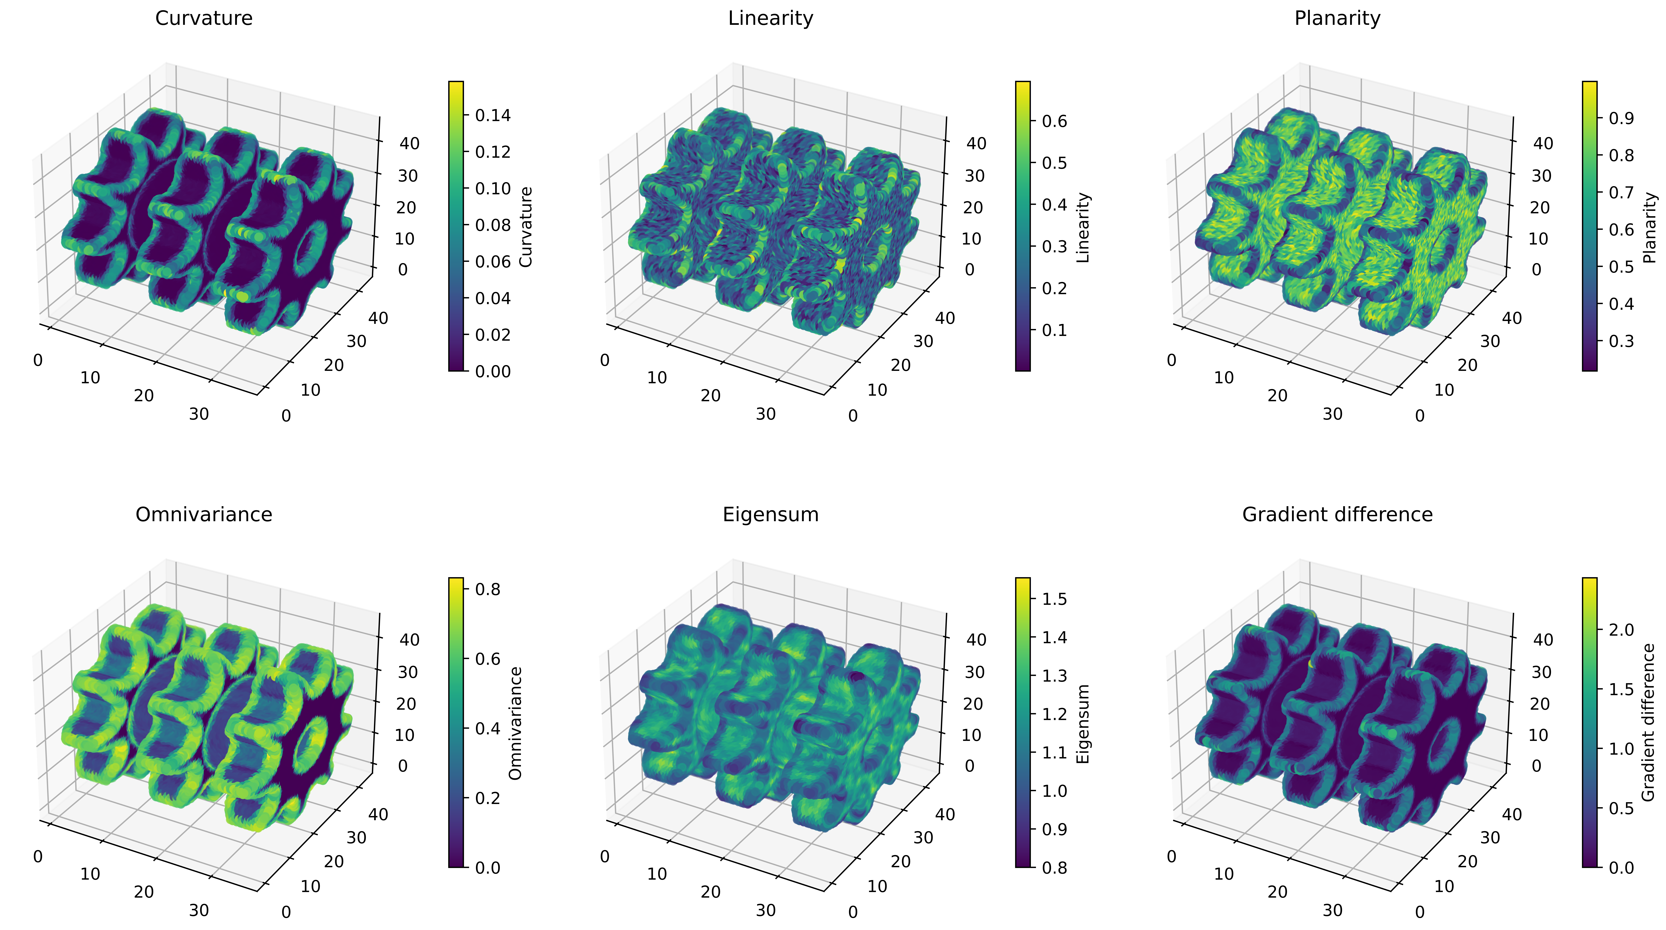
\includegraphics[width=\textwidth]{figures/feature_plots_lowQ.png}
    \caption{Geometry bias features}\label{fig:feature_plot}
\end{figure*}

\subsection*{Final Feature Set}
The features used for training the final model was.
\begin{itemize}
    \item Average Radius
    \item Points inside
    \item Curvature
    \item Linearity
    \item Planarity
    \item Gradient Difference
\end{itemize}
\vspace{5pt}

The feature correlation matrix, shown in Figure \ref{fig:feature_correlation}, provides insight into the linear relationships between the input features used for training. In general, moderate correlations indicate that each feature captures distinct aspects of local geometry, supporting the robustness of the final feature set. A notable observation is the very strong negative correlation (-0.96) between linearity and planarity, suggesting these two features capture highly similar structural information in different ways. However, both are included in the feature set because they emphasize different aspects of local structure—linearity highlights edge-like features, while planarity captures flatness. Including both ensures that the model has access to these complementary geometric cues, even if their numerical values are strongly linked.
\begin{figure}[htbp]
    \centering
    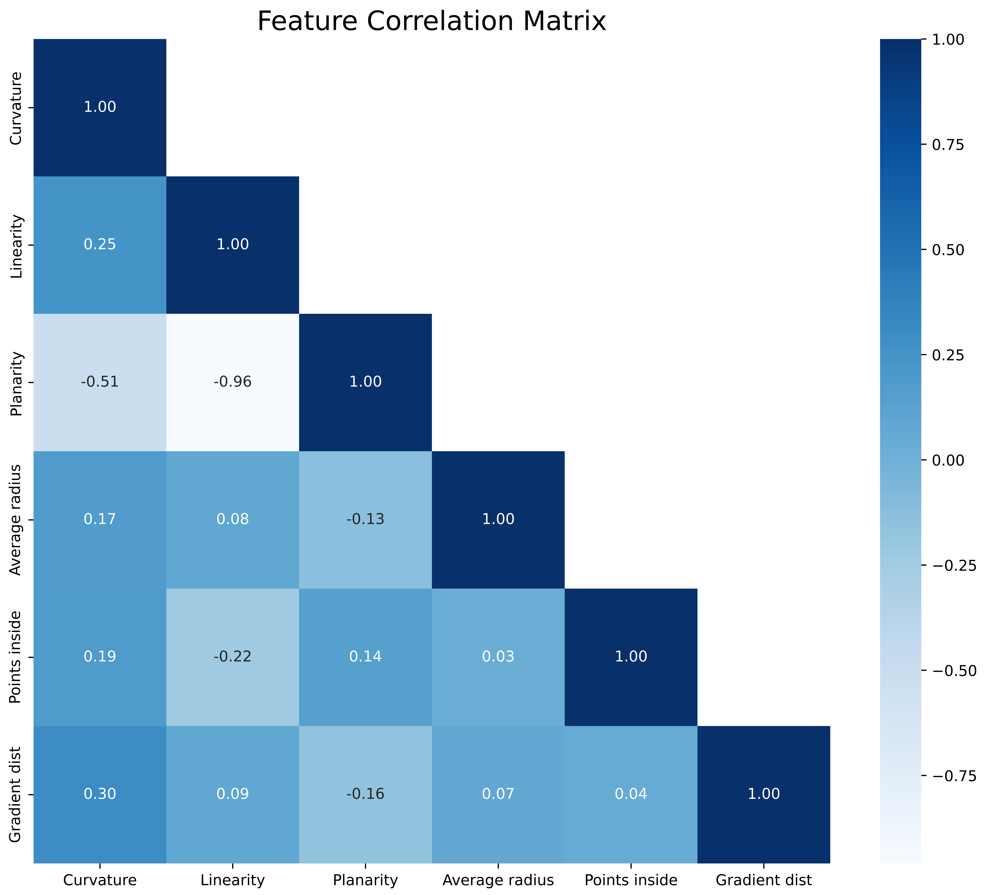
\includegraphics[width=0.4\textwidth]{figures/correlation_matrix_final_lowQ.png}
    \caption{Correlation matrix between features}
    \label{fig:feature_correlation}
\end{figure}
<<<<<<< Updated upstream
<\subsection{Neaural Network}
The neural network model is a Multi-Layer Perceptron (MLP) designed to predict the quality of pointclouds based on their extracted features. The architecture consists of an input layer, four hidden layers, and an output layer. The hidden layers have 64, 128, 128, and 64 units, respectively, and use the ReLU activation function to introduce non-linearity. The output layer consists of a single unit that produces the final prediction. The model is implemented using the FLAX NNX framework, which is part of the JAX ecosystem, enabling efficient automatic differentiation and GPU acceleration. Training is performed using the Adam optimizer with a learning rate of 0.001 and a large batch size of 200,000. The network minimizes the mean squared error (MSE) between the predicted values and the ground truth, and is trained for 1000 epochs.

The features are standardized before being fed into the model and 80\% of the data is used for training, while 20\% is reserved for validation. This ensures that the model generalizes well to unseen data. 


\begin{table}[htbp]
\centering
\begin{tabular}{|l|c|c|}
\hline
\textbf{Score} & \textbf{Small model} & \textbf{Big model} \\
\hline
R\textsuperscript{2} & 0.9818 & 0.9910 \\
MAE & 0.0425 & 0.0318 \\
MSE & 0.0137 & 0.0068 \\
RMSE & 0.1170 & 0.0825 \\
Max error & 1.8672 & 1.6806 \\
\hline
\end{tabular}
\vspace{0.5em}  % Adjust as needed
\caption{Comparison of model evaluation metrics between models.}
\label{tab:model_metrics}
\end{table}
=======
\subsection{Neaural Network}
>>>>>>> Stashed changes


\section{Experiments}
\subsection{Datasets}
Accurate point clouds are crucial to ensure that the predictions made by the model are built upon a reliable foundation. To generate synthetic “perfect” point clouds, parametric geometries were created in SolidWorks, introducing various shapes composed of simple geometries (see Figure \ref{fig:part_shapes_grid}). The parametric definitions of these geometries allow for the creation of numerous variations for each shape, resulting in a vast amount of data. Specifically, each part is represented in four different variations. These geometries are then converted into point clouds using \texttt{MeshLab}. A Poisson disc sampling technique is employed to ensure that the point clouds are uniformly distributed. To further enhance the robustness of the model, imperfections are deliberately introduced into the point clouds. By creating holes within the generated point clouds, the dataset will contain a mixture of points that are perfect and points that are in a low surface density area. 

After pointclouds are generated, features are extracted for each pointcloud using the method described in Section \ref{sec:features}. The labels are calculated by extracting the surface area of the parts from Solidworks and dividing it by the number of points in the pointcloud. This label is attached to all points in the pointcloud and only changed for points that are next to a generated hole. For points next to a hole, the surface density is halved to better match the ground truth quality of the point neighborhood.

The method was used to generate two datasets:
\begin{itemize}
    \item \textbf{Dataset 1 (Coarse mesh sampling)}: Mesh sizes of 0.5\,mm, 1\,mm, and 2\,mm were used for sampling the geometries, resulting in a dataset of 1,562,211 points.
    
    \item \textbf{Dataset 2 (Fine mesh sampling)}: Mesh sizes from 0.5\,mm to 2\,mm were generated at 0.1\,mm intervals, producing a finely sampled dataset of 4,950,604 points. This dataset allows the model to experience a smooth transition in mesh resolution, enhancing its ability to handle diverse point densities.
\end{itemize}



\begin{figure}[htbp]
  \centering
  \begin{minipage}{0.5\textwidth} % Half page width
    \centering
    \setlength{\tabcolsep}{1pt}
    \renewcommand{\arraystretch}{0.9}

    \begin{tabular}{ccc}
      \begin{minipage}{0.3\linewidth}
        \centering
        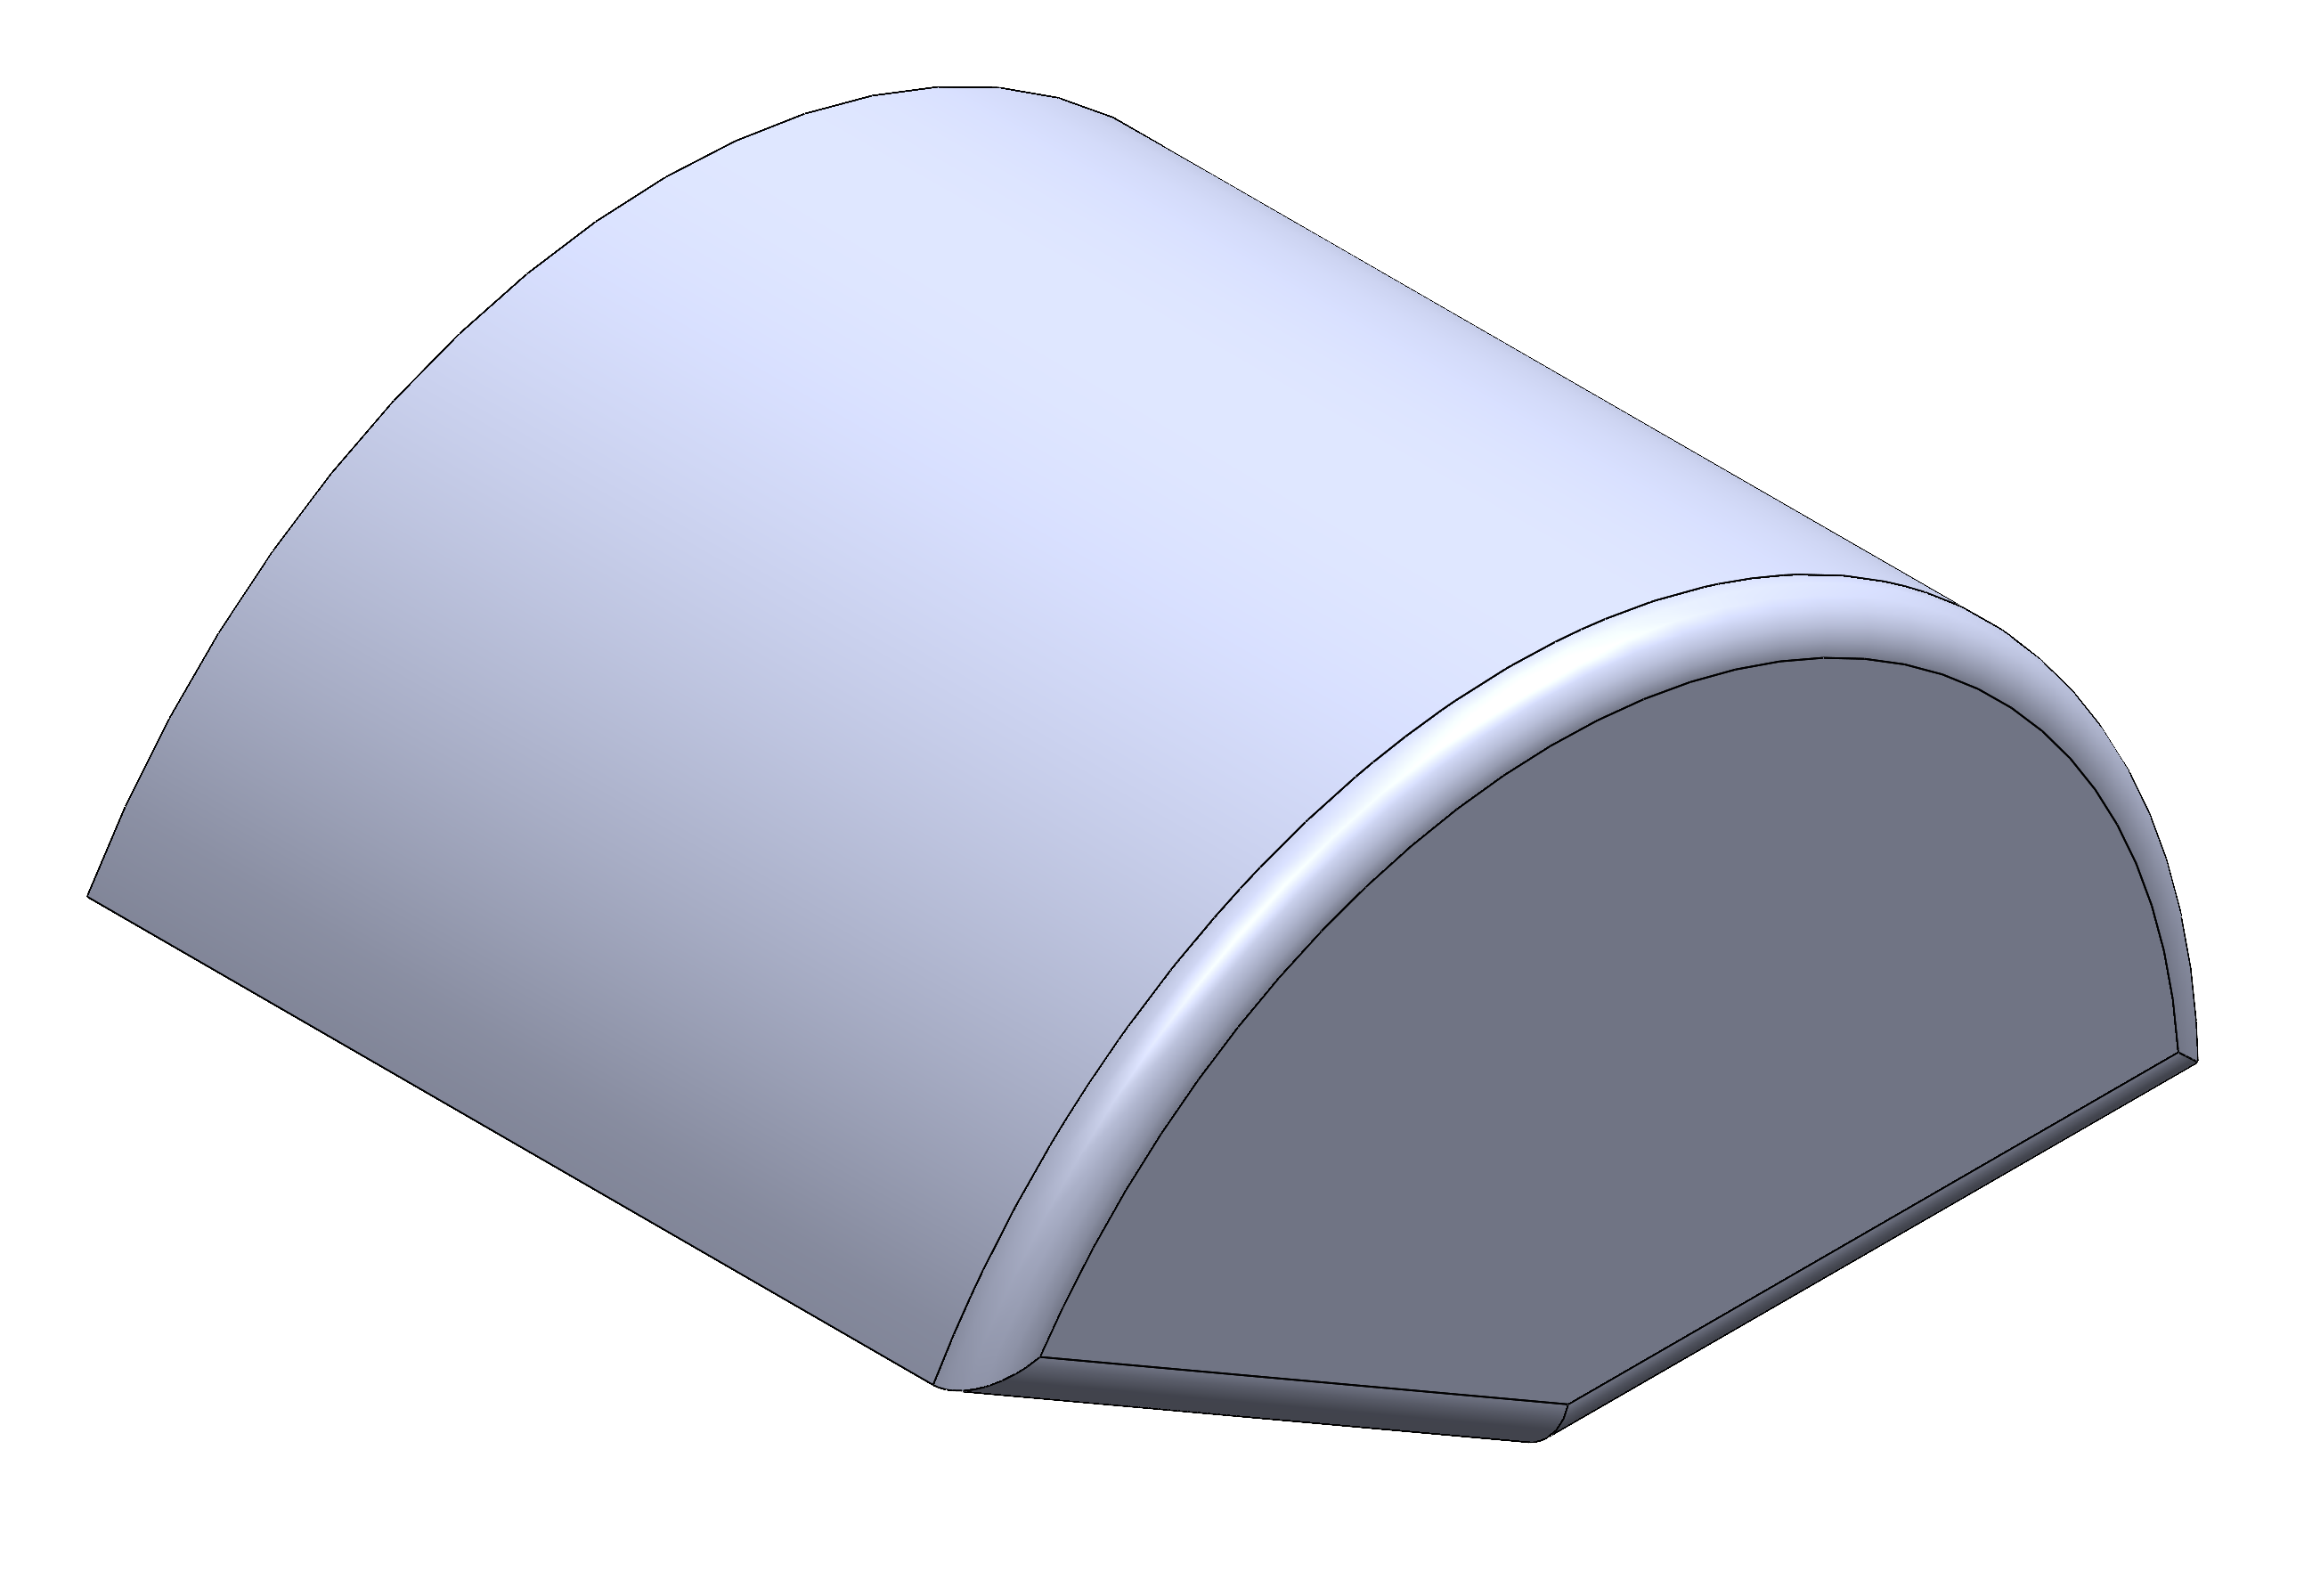
\includegraphics[width=\linewidth]{figures/parts/angle_curve.PNG}
        \scriptsize Angle Curve
      \end{minipage} &
      \begin{minipage}{0.3\linewidth}
        \centering
        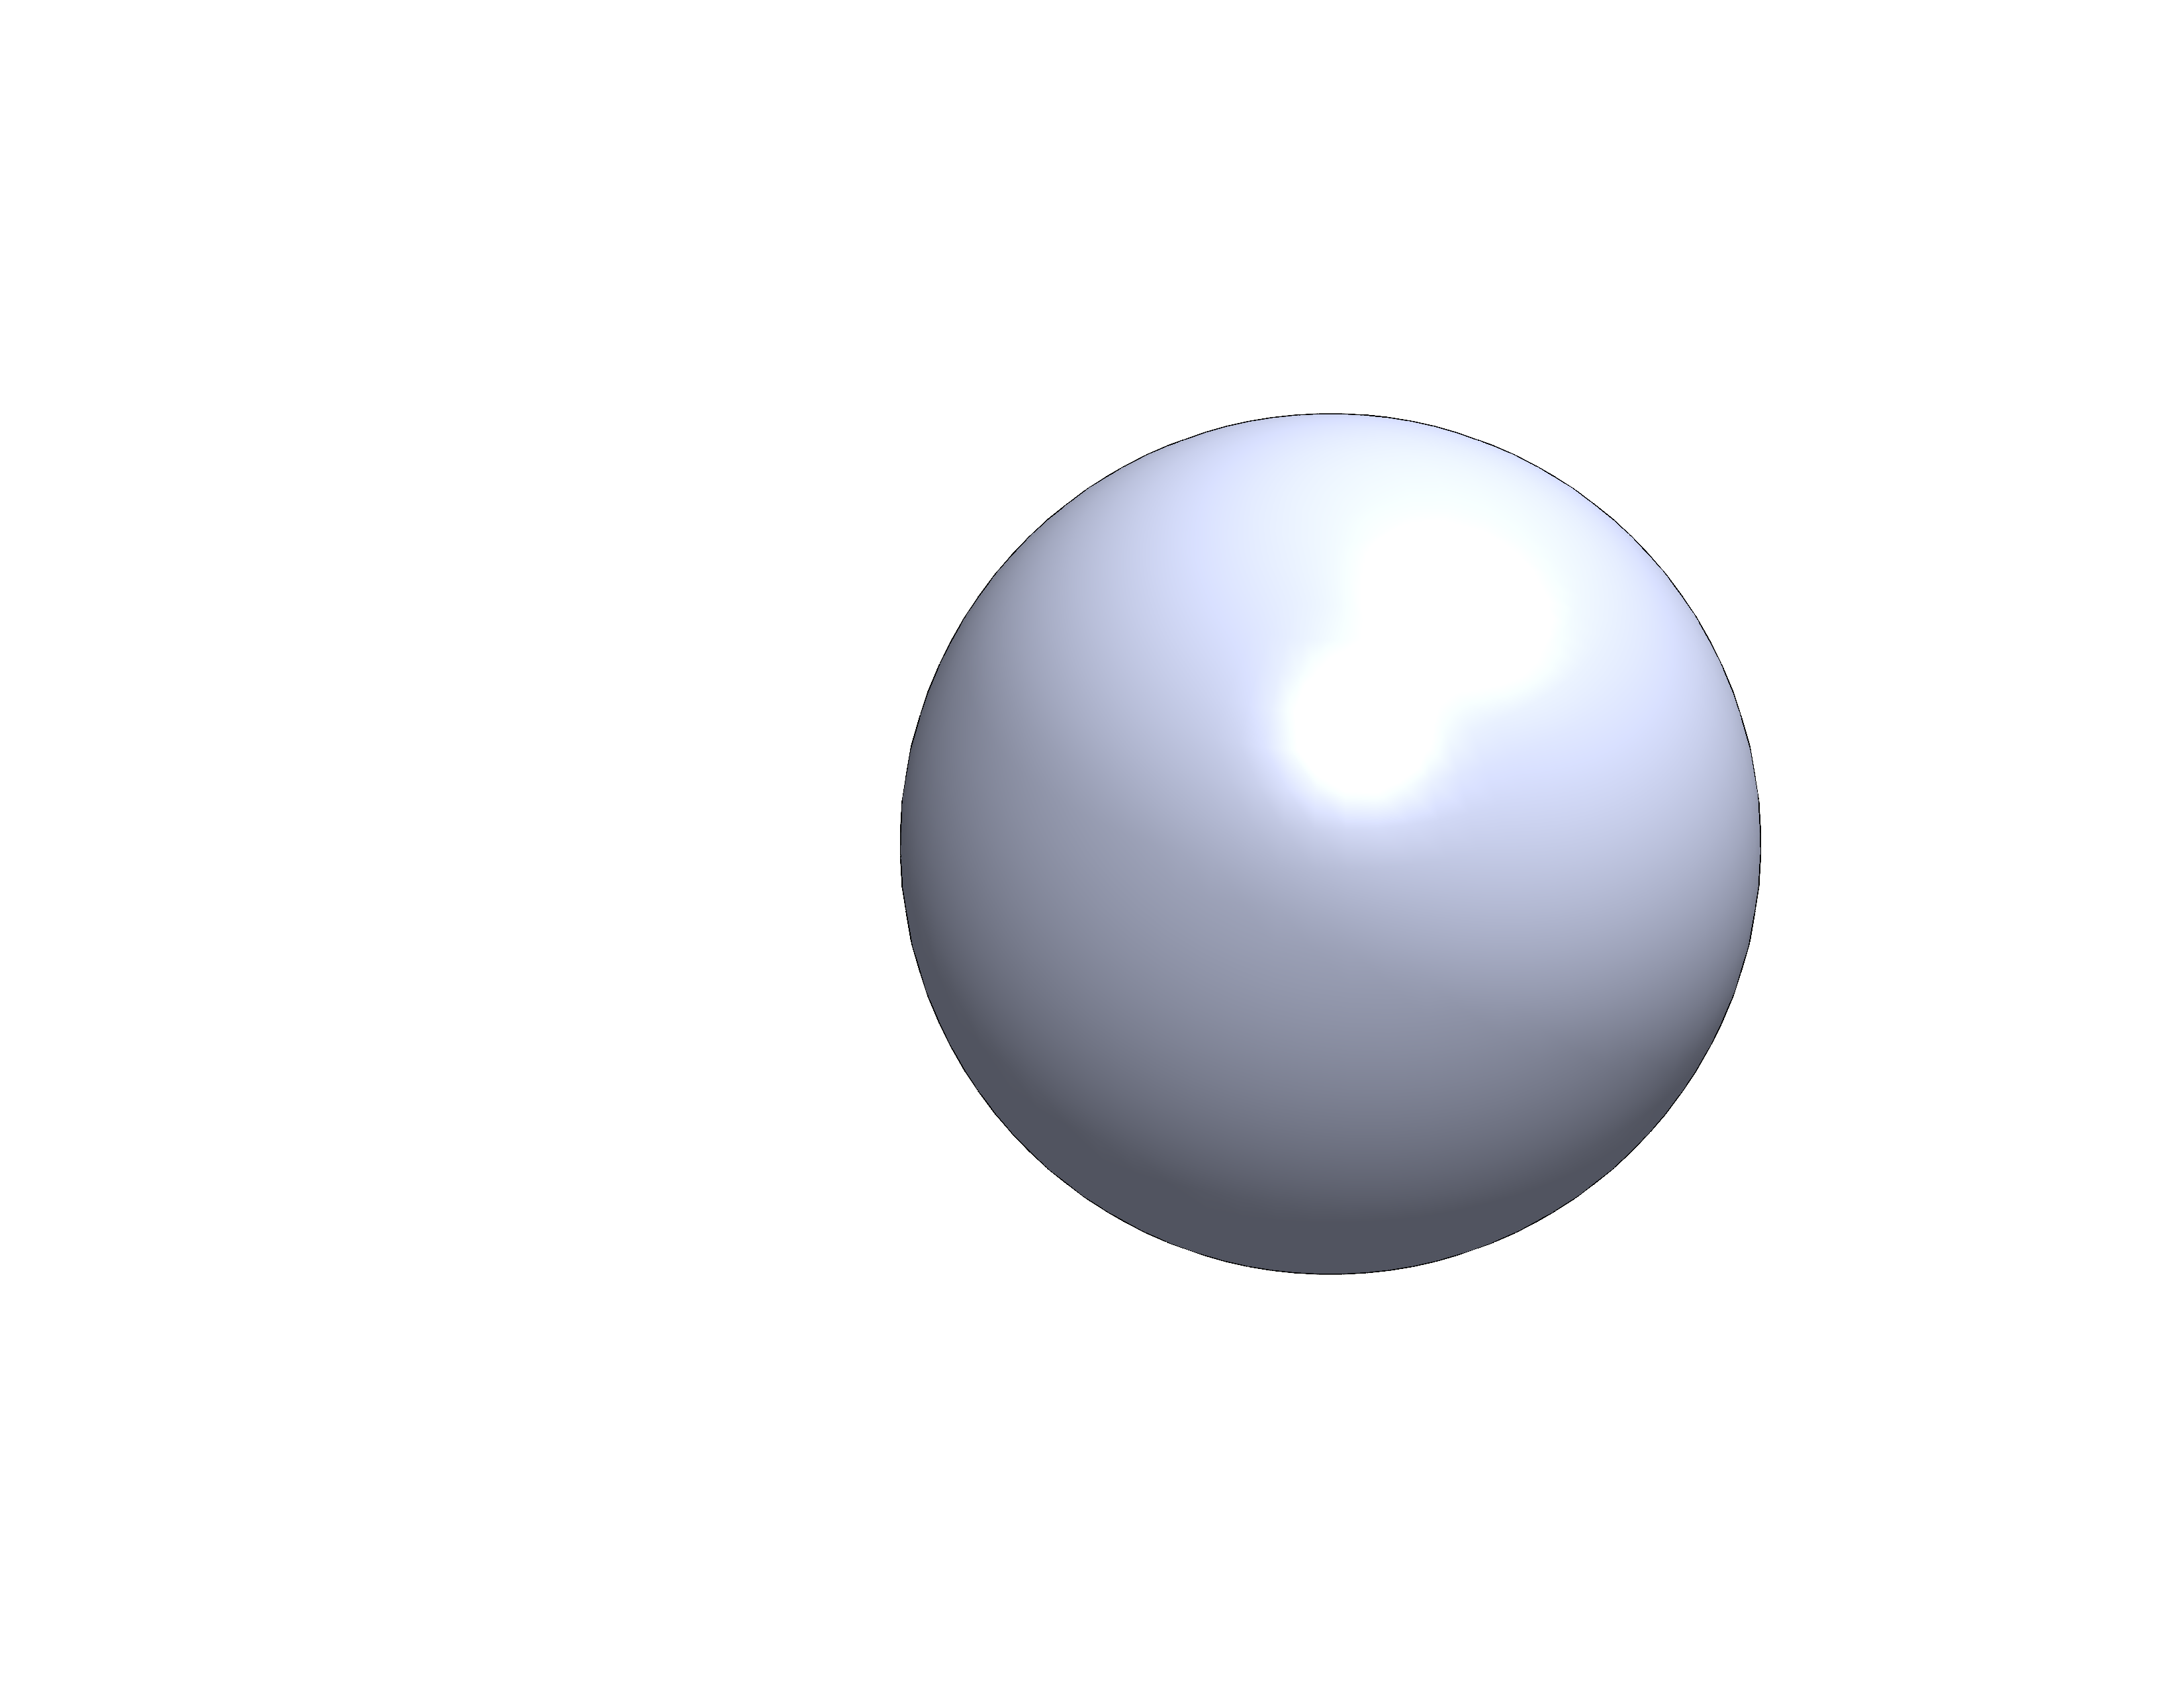
\includegraphics[width=\linewidth]{figures/parts/Ball.PNG}
        \scriptsize     Ball
      \end{minipage} &
      \begin{minipage}{0.3\linewidth}
        \centering
        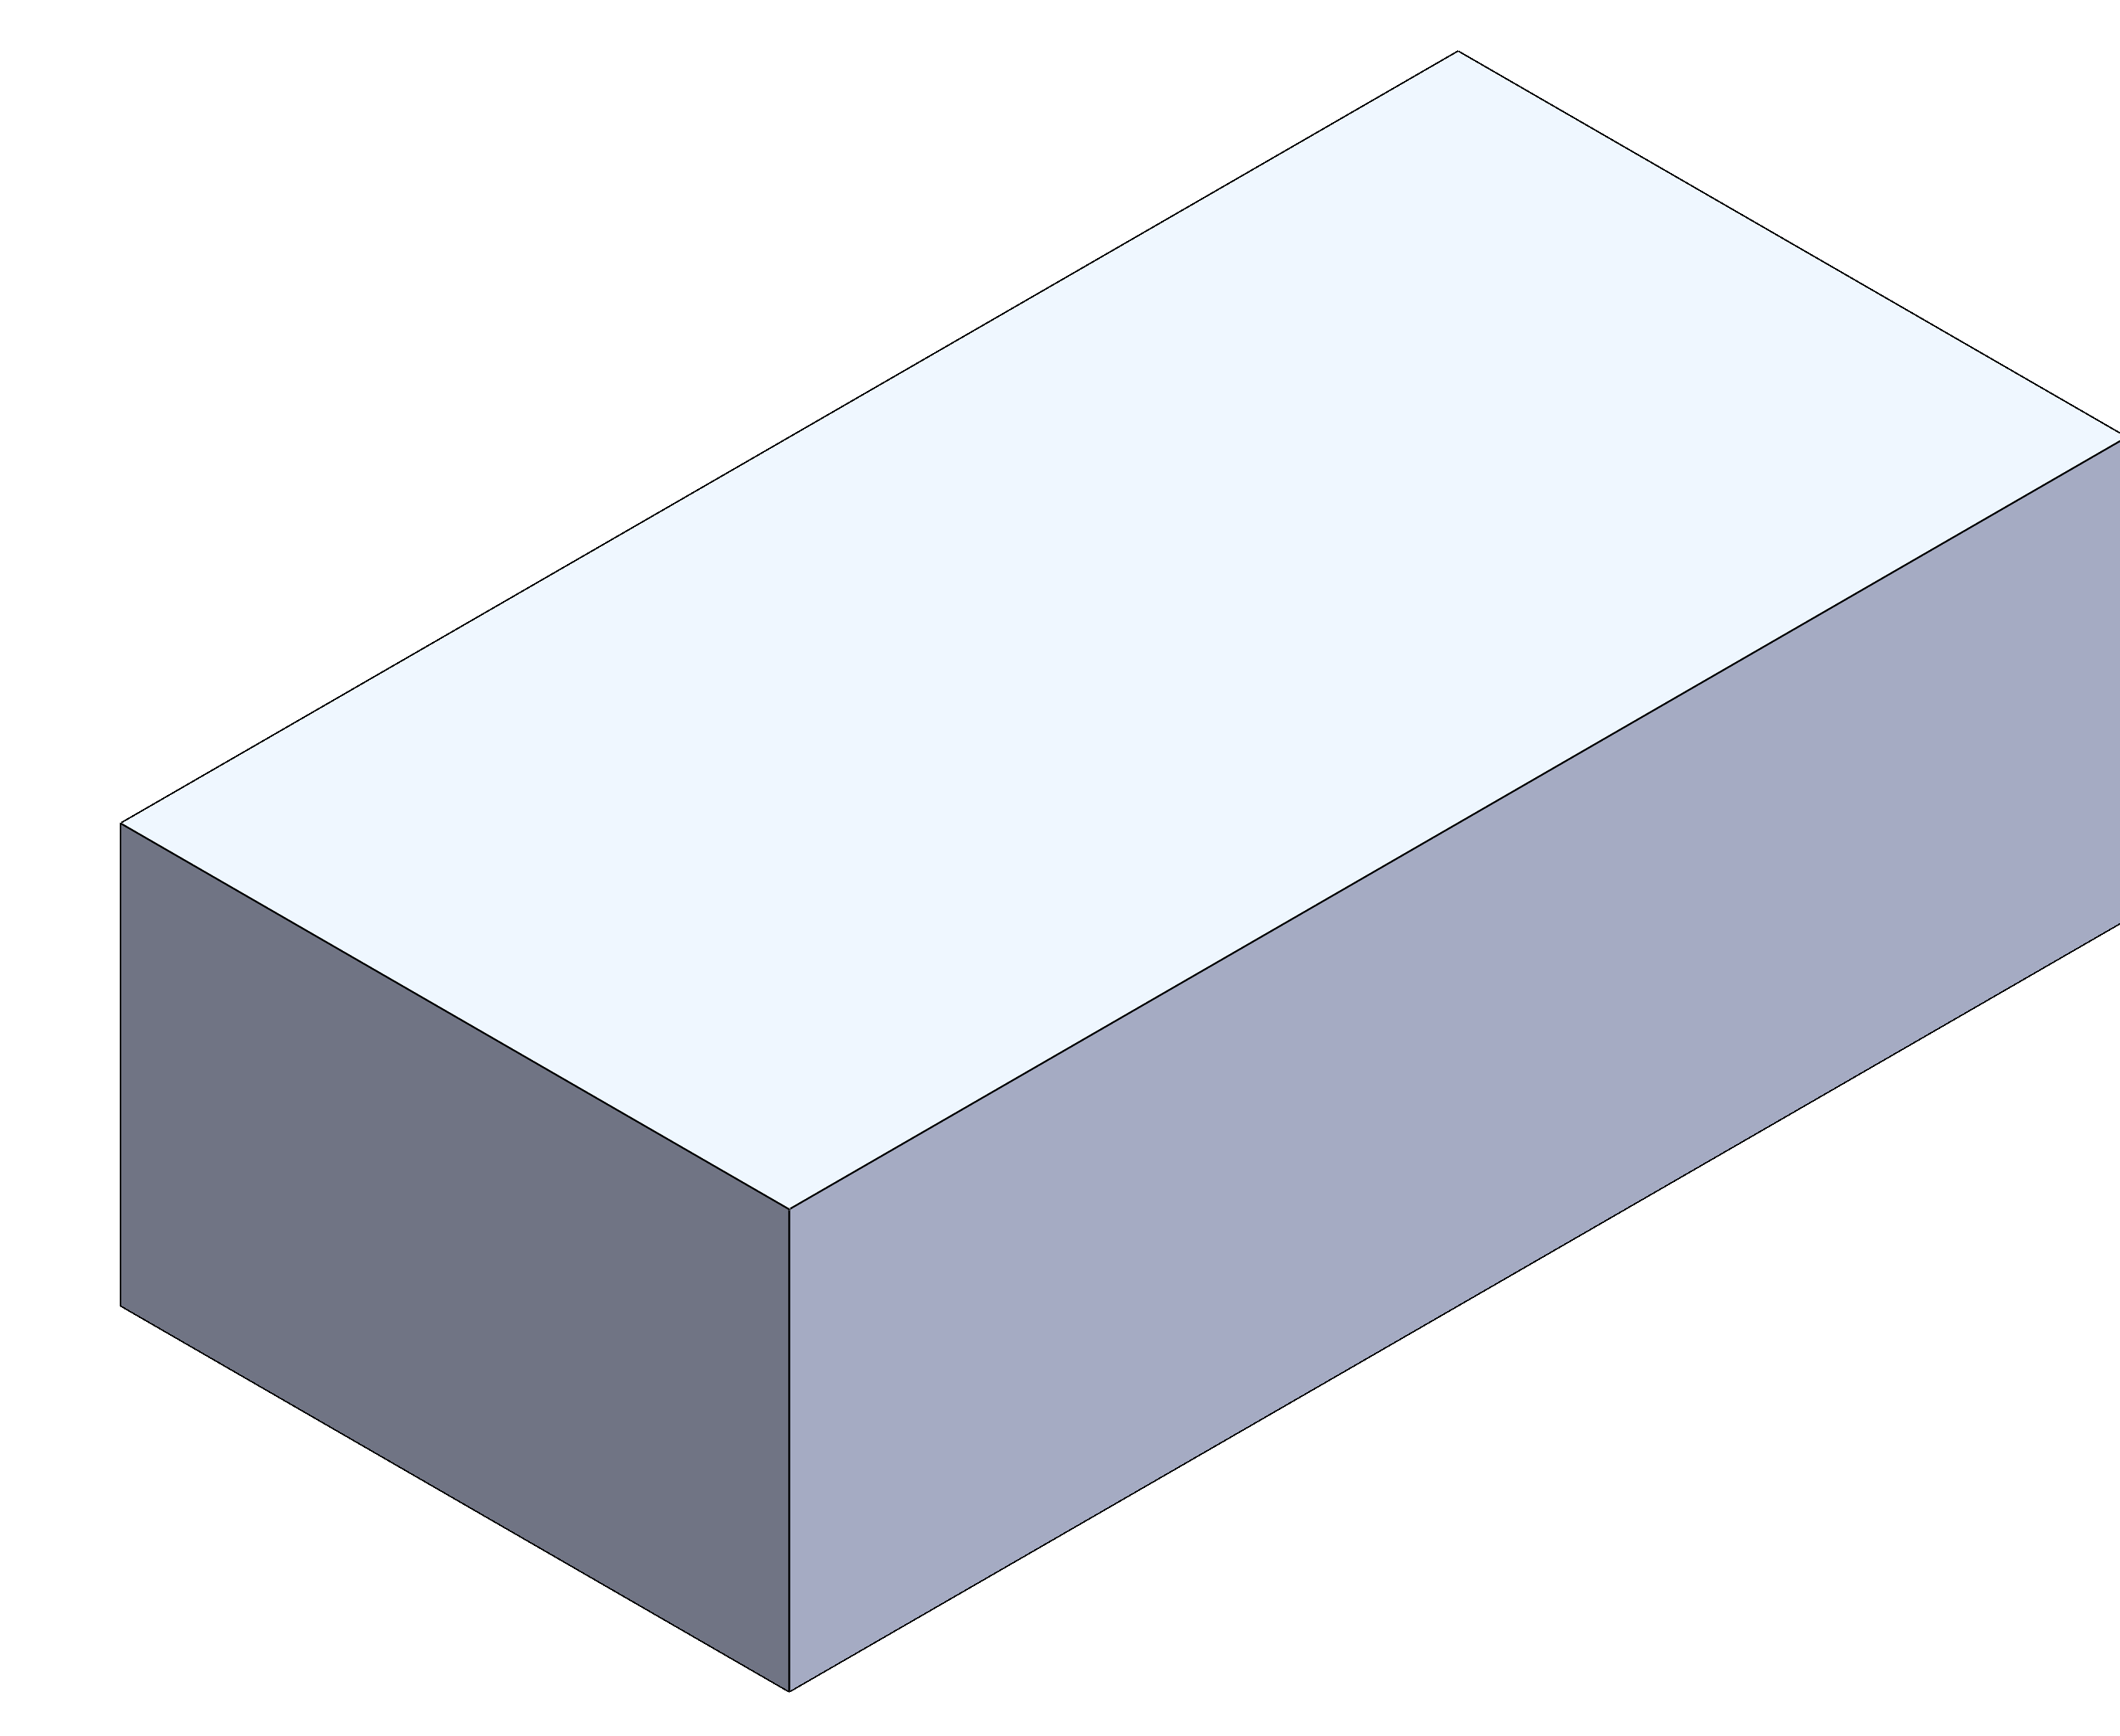
\includegraphics[width=\linewidth]{figures/parts/Box.PNG}
        \scriptsize Box
      \end{minipage} \\

      \begin{minipage}{0.3\linewidth}
        \centering
        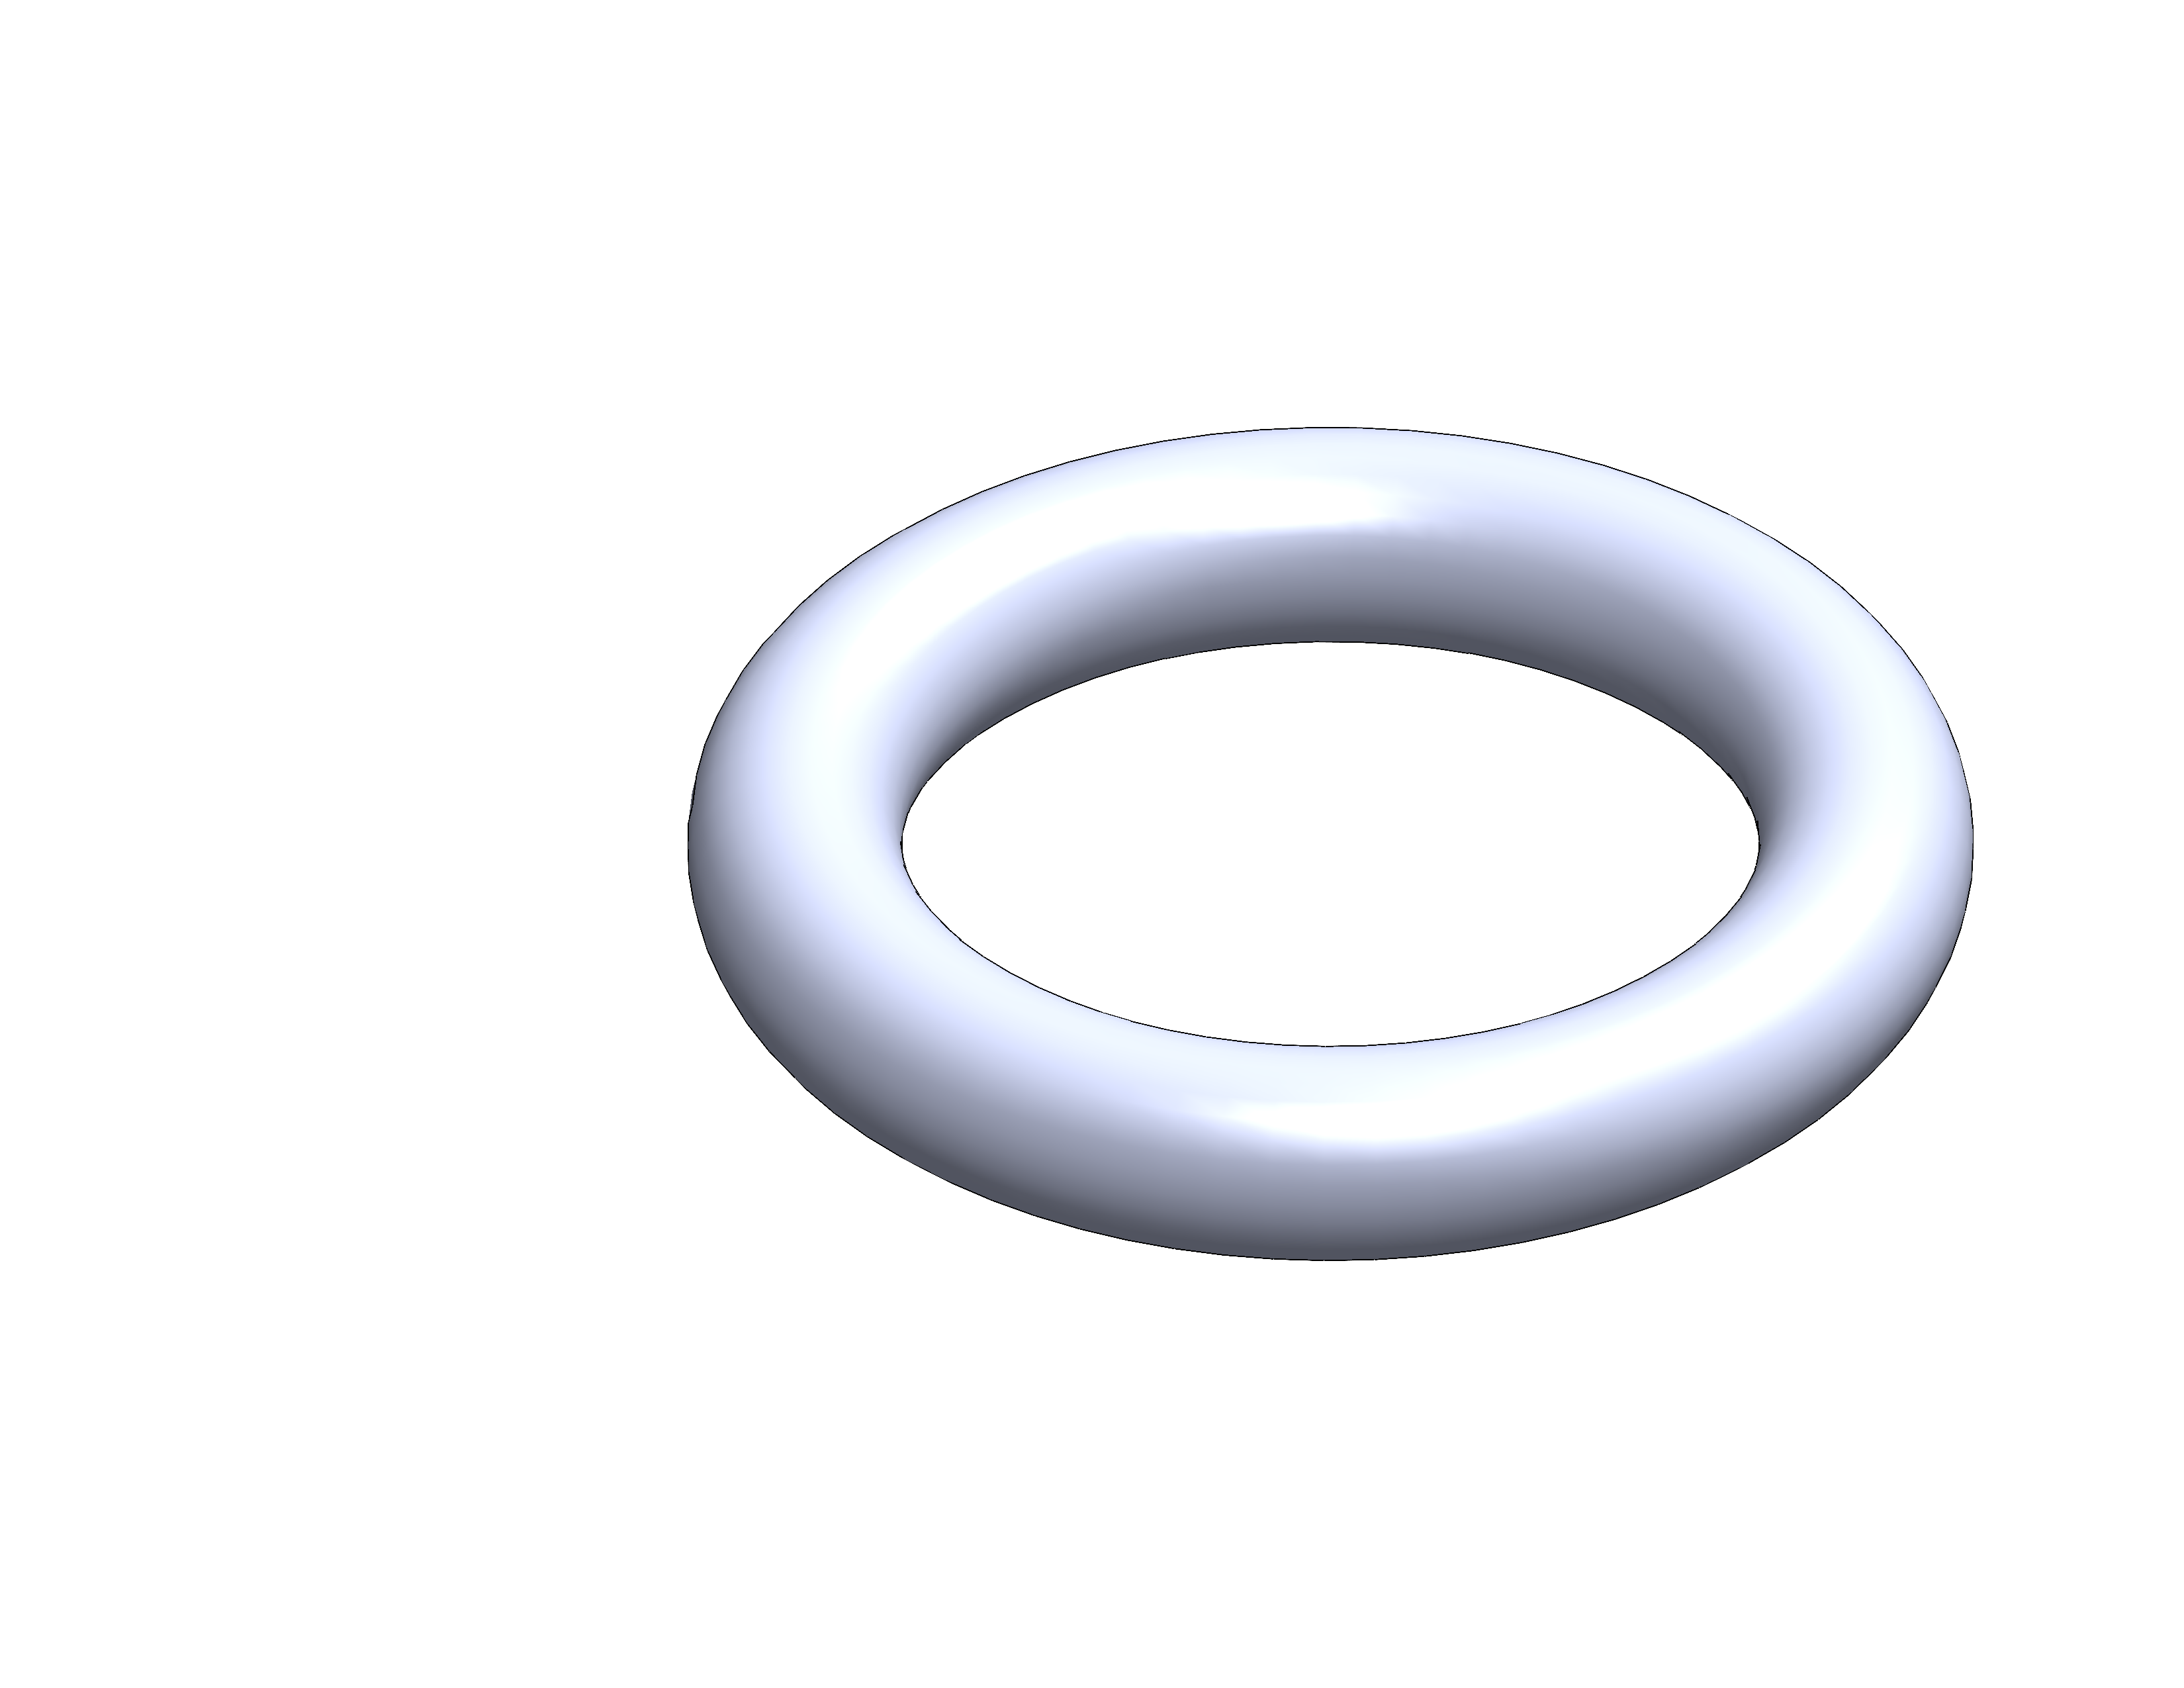
\includegraphics[width=\linewidth]{figures/parts/donut.PNG}
        \scriptsize Donut
      \end{minipage} &
      \begin{minipage}{0.3\linewidth}
        \centering
        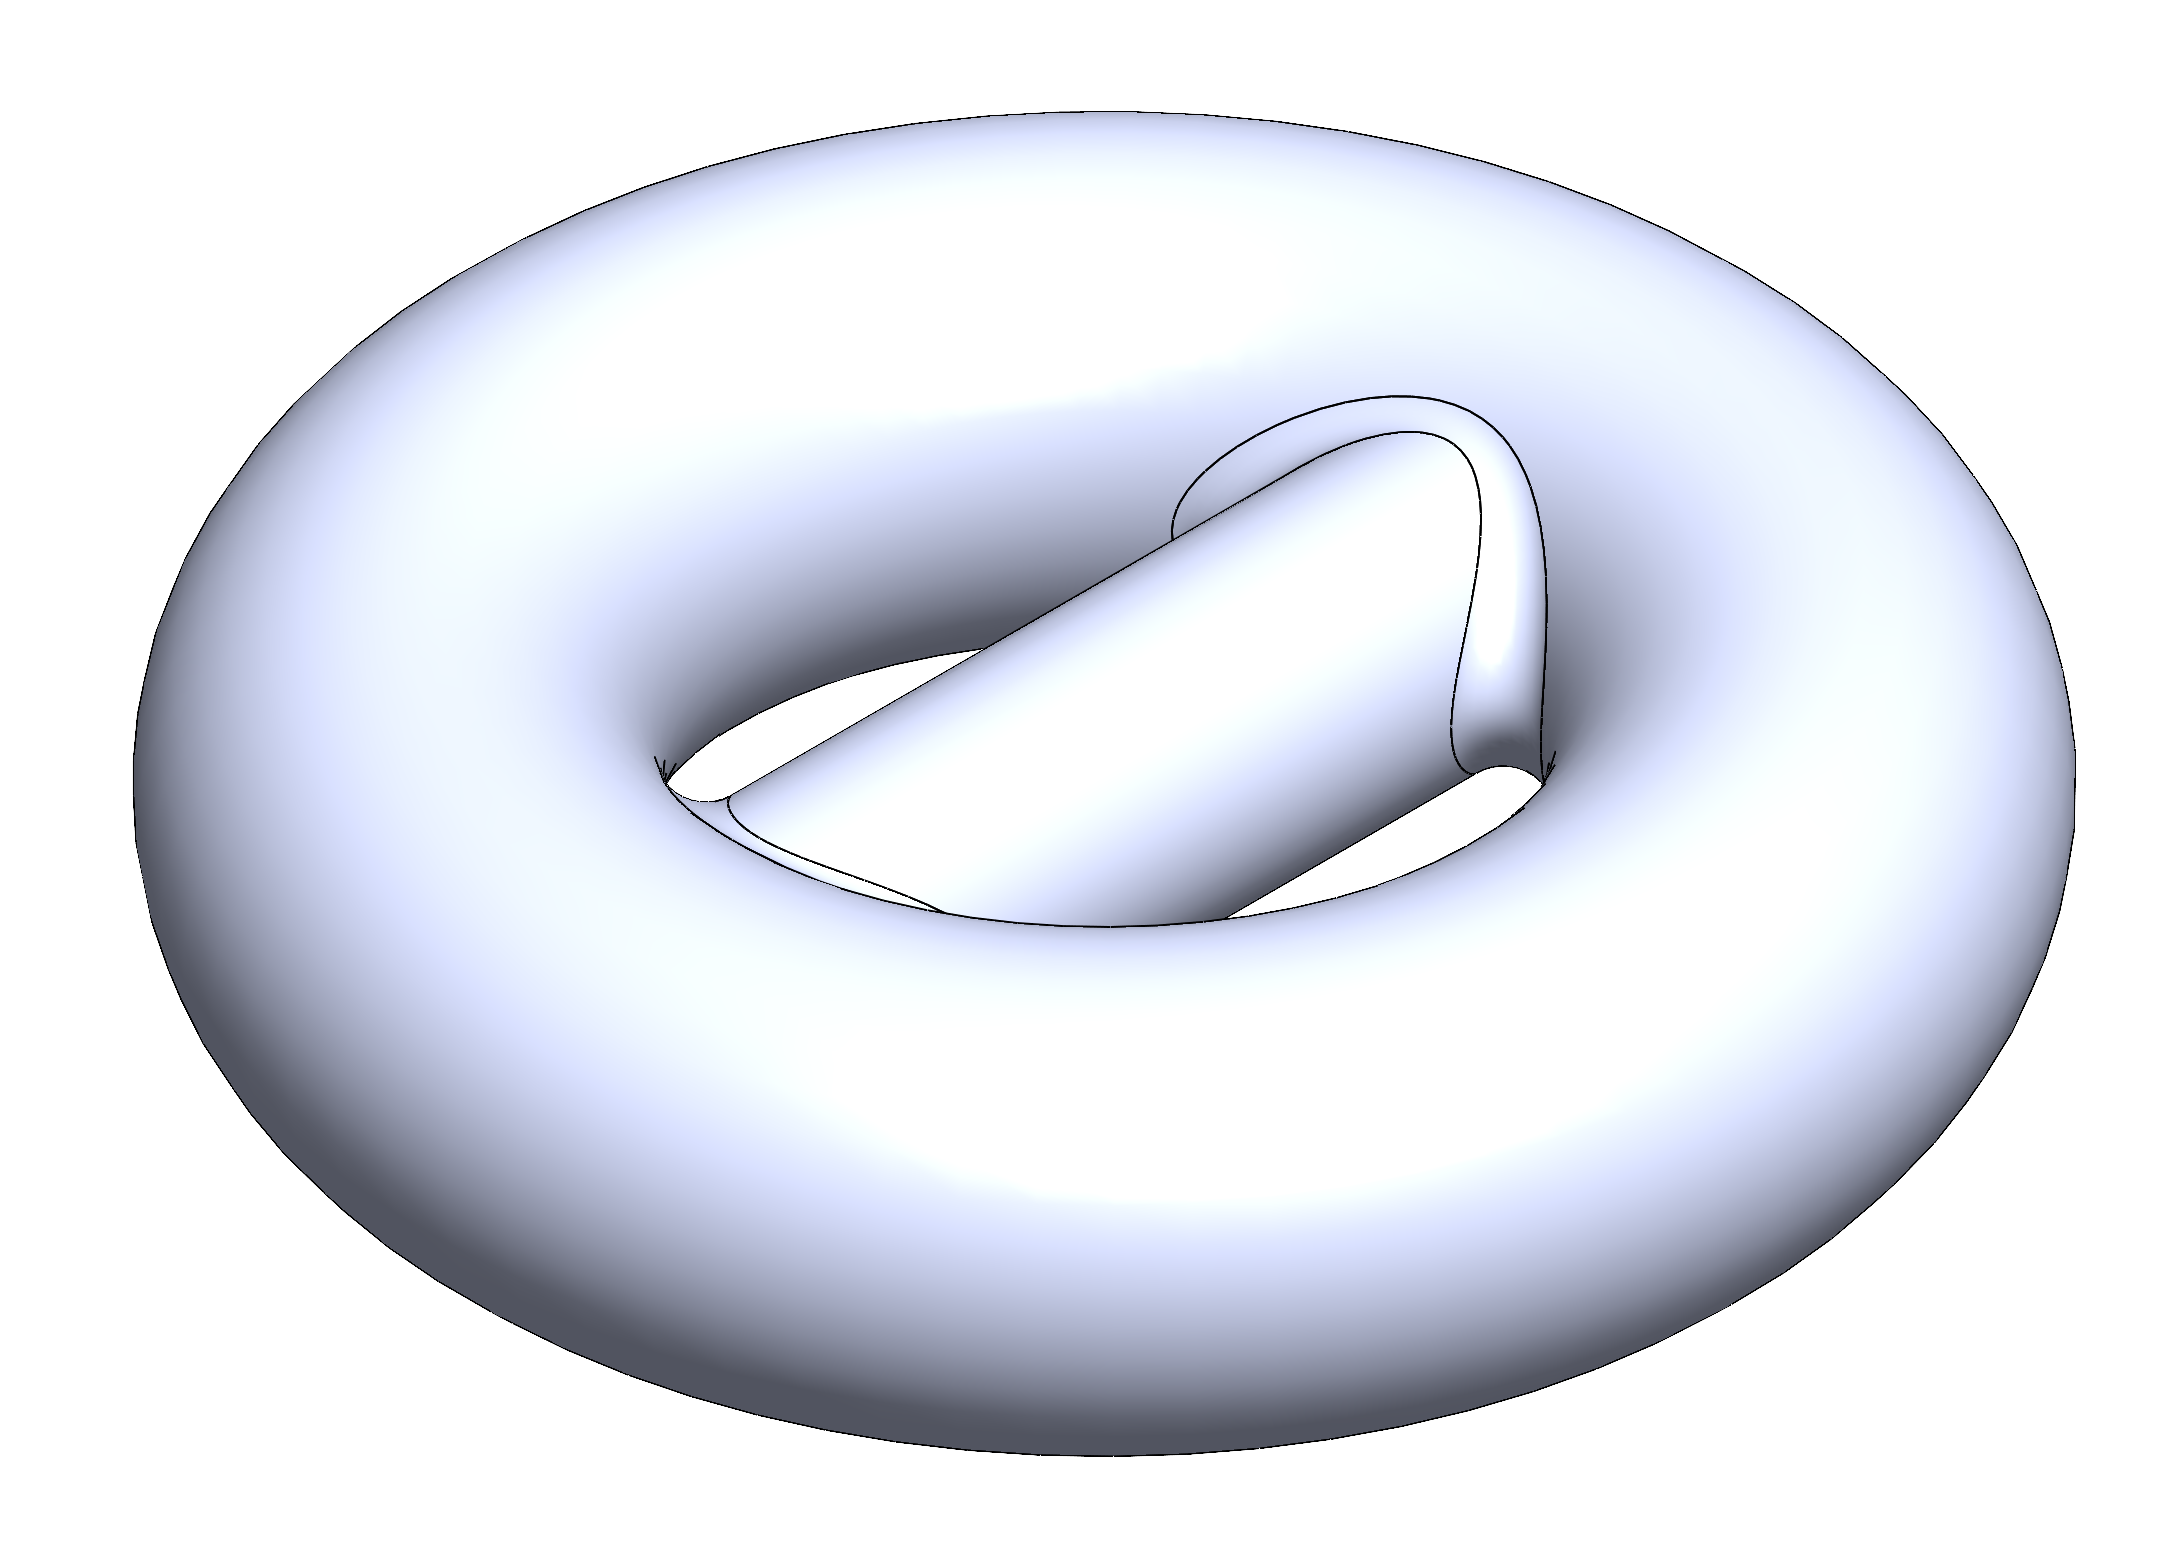
\includegraphics[width=\linewidth]{figures/parts/Donut_w_center.PNG}
        \scriptsize Donut w/ Center
      \end{minipage} &
      \begin{minipage}{0.3\linewidth}
        \centering
        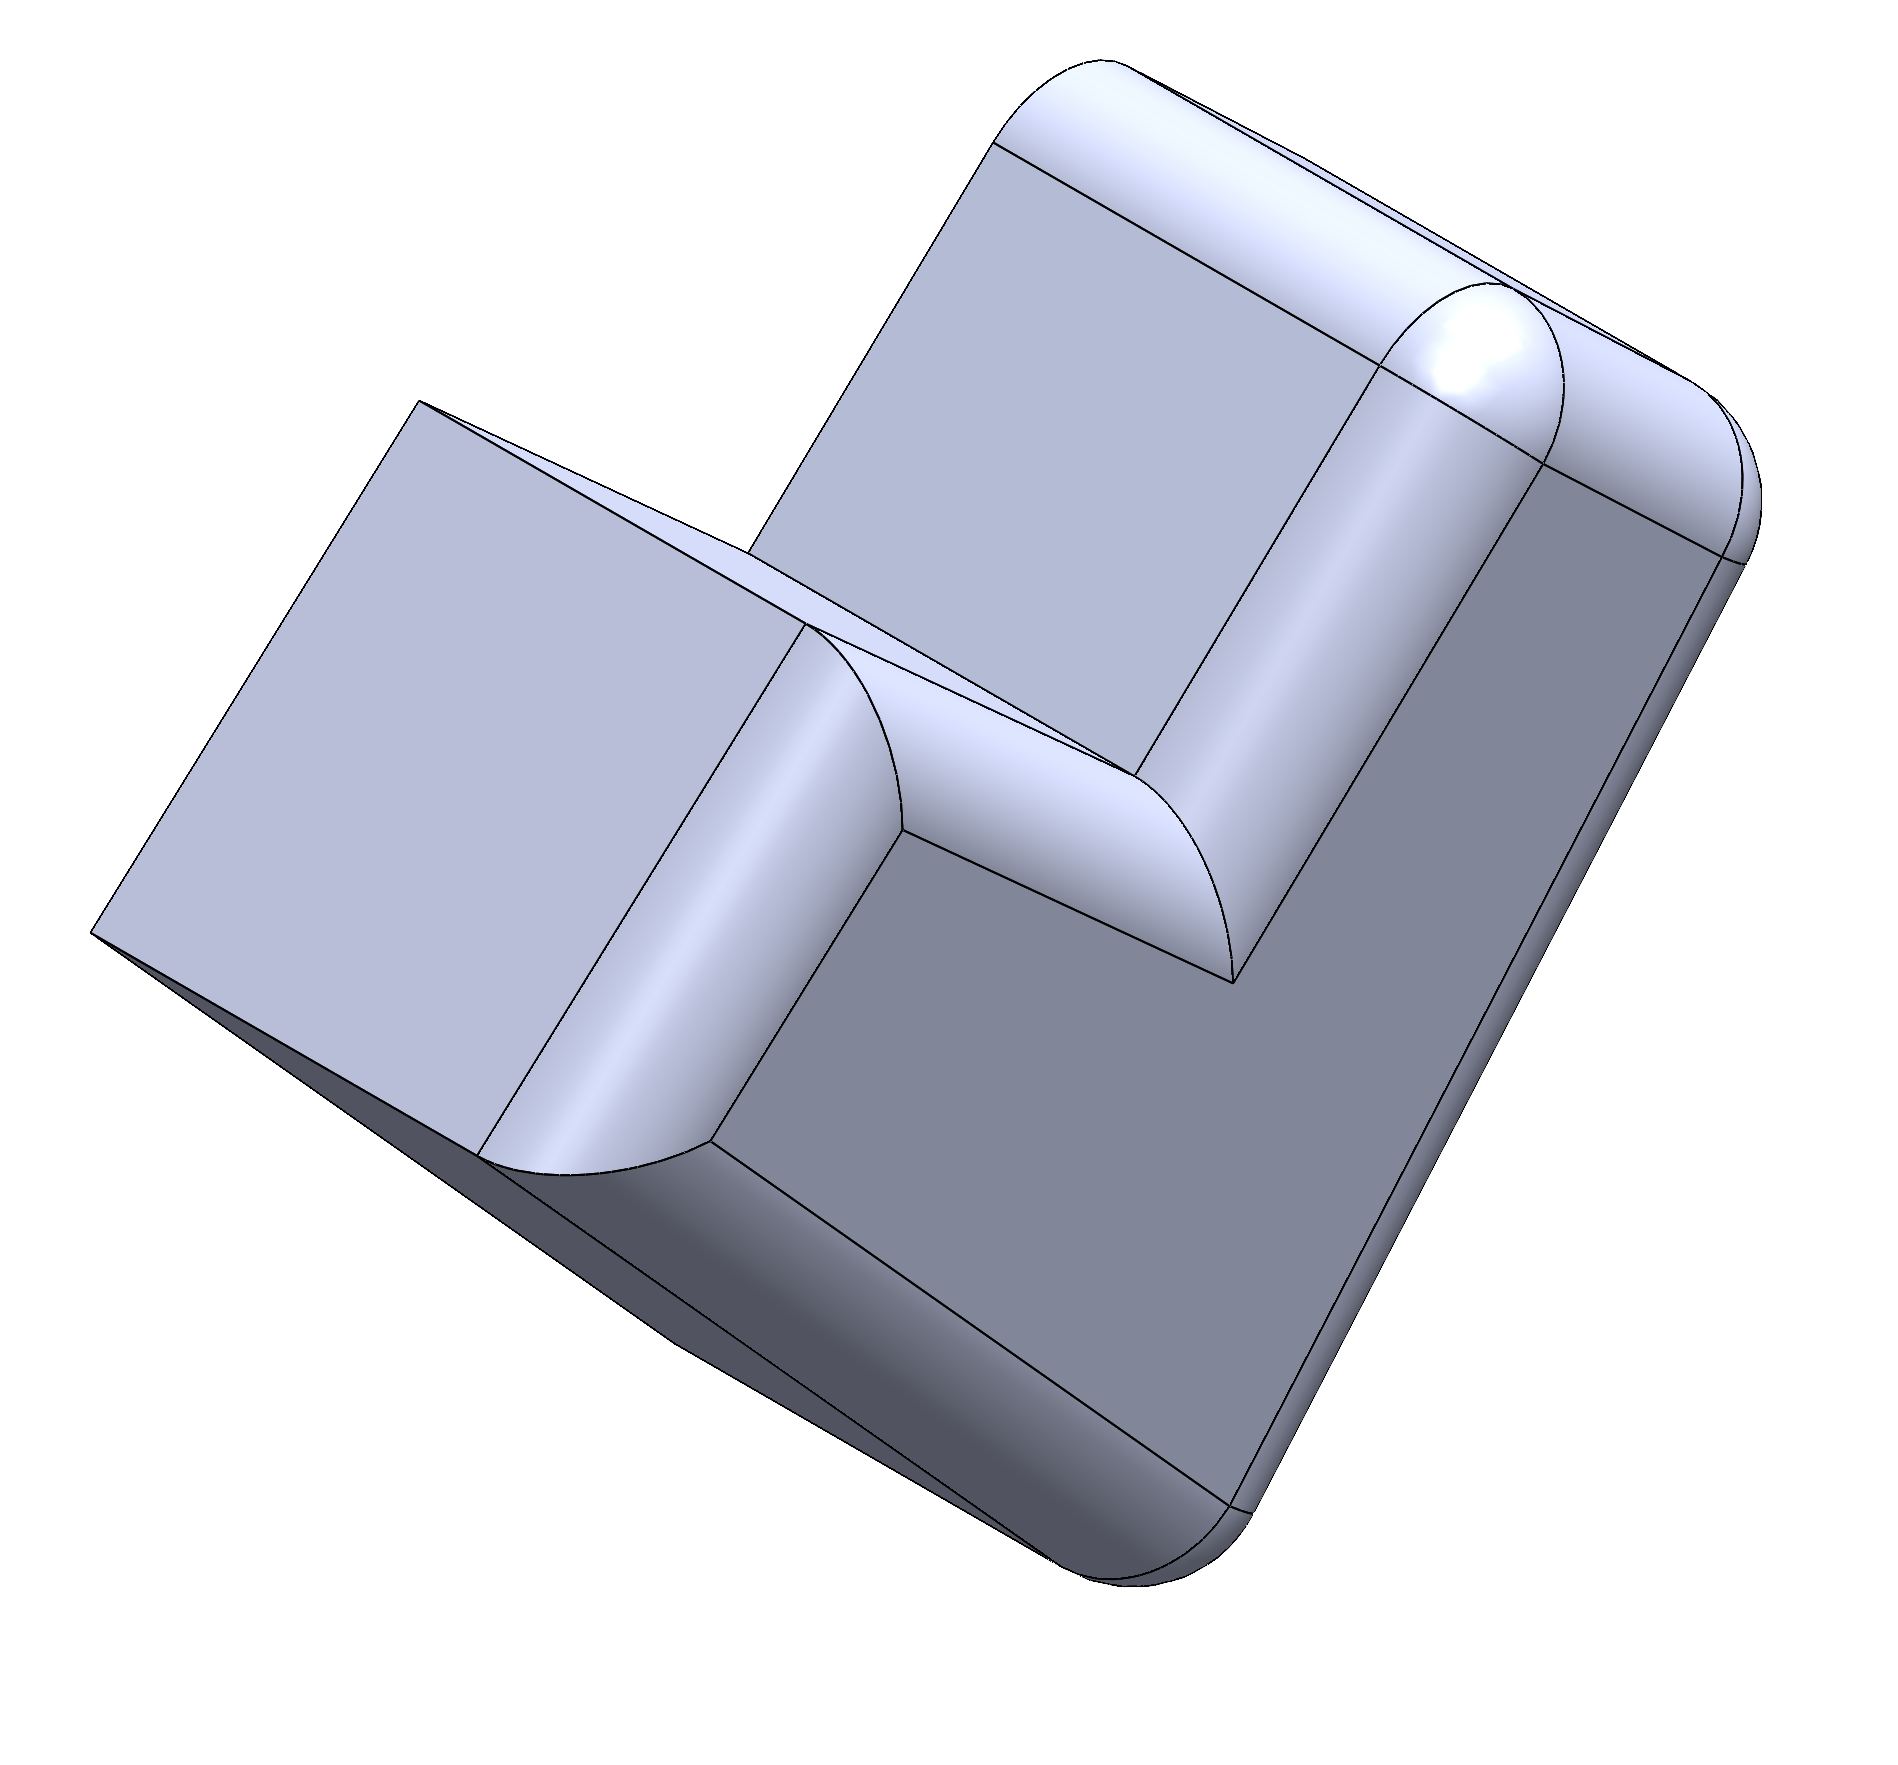
\includegraphics[width=\linewidth]{figures/parts/heart.PNG}
        \scriptsize Heart
      \end{minipage} \\

      \begin{minipage}{0.3\linewidth}
        \centering
        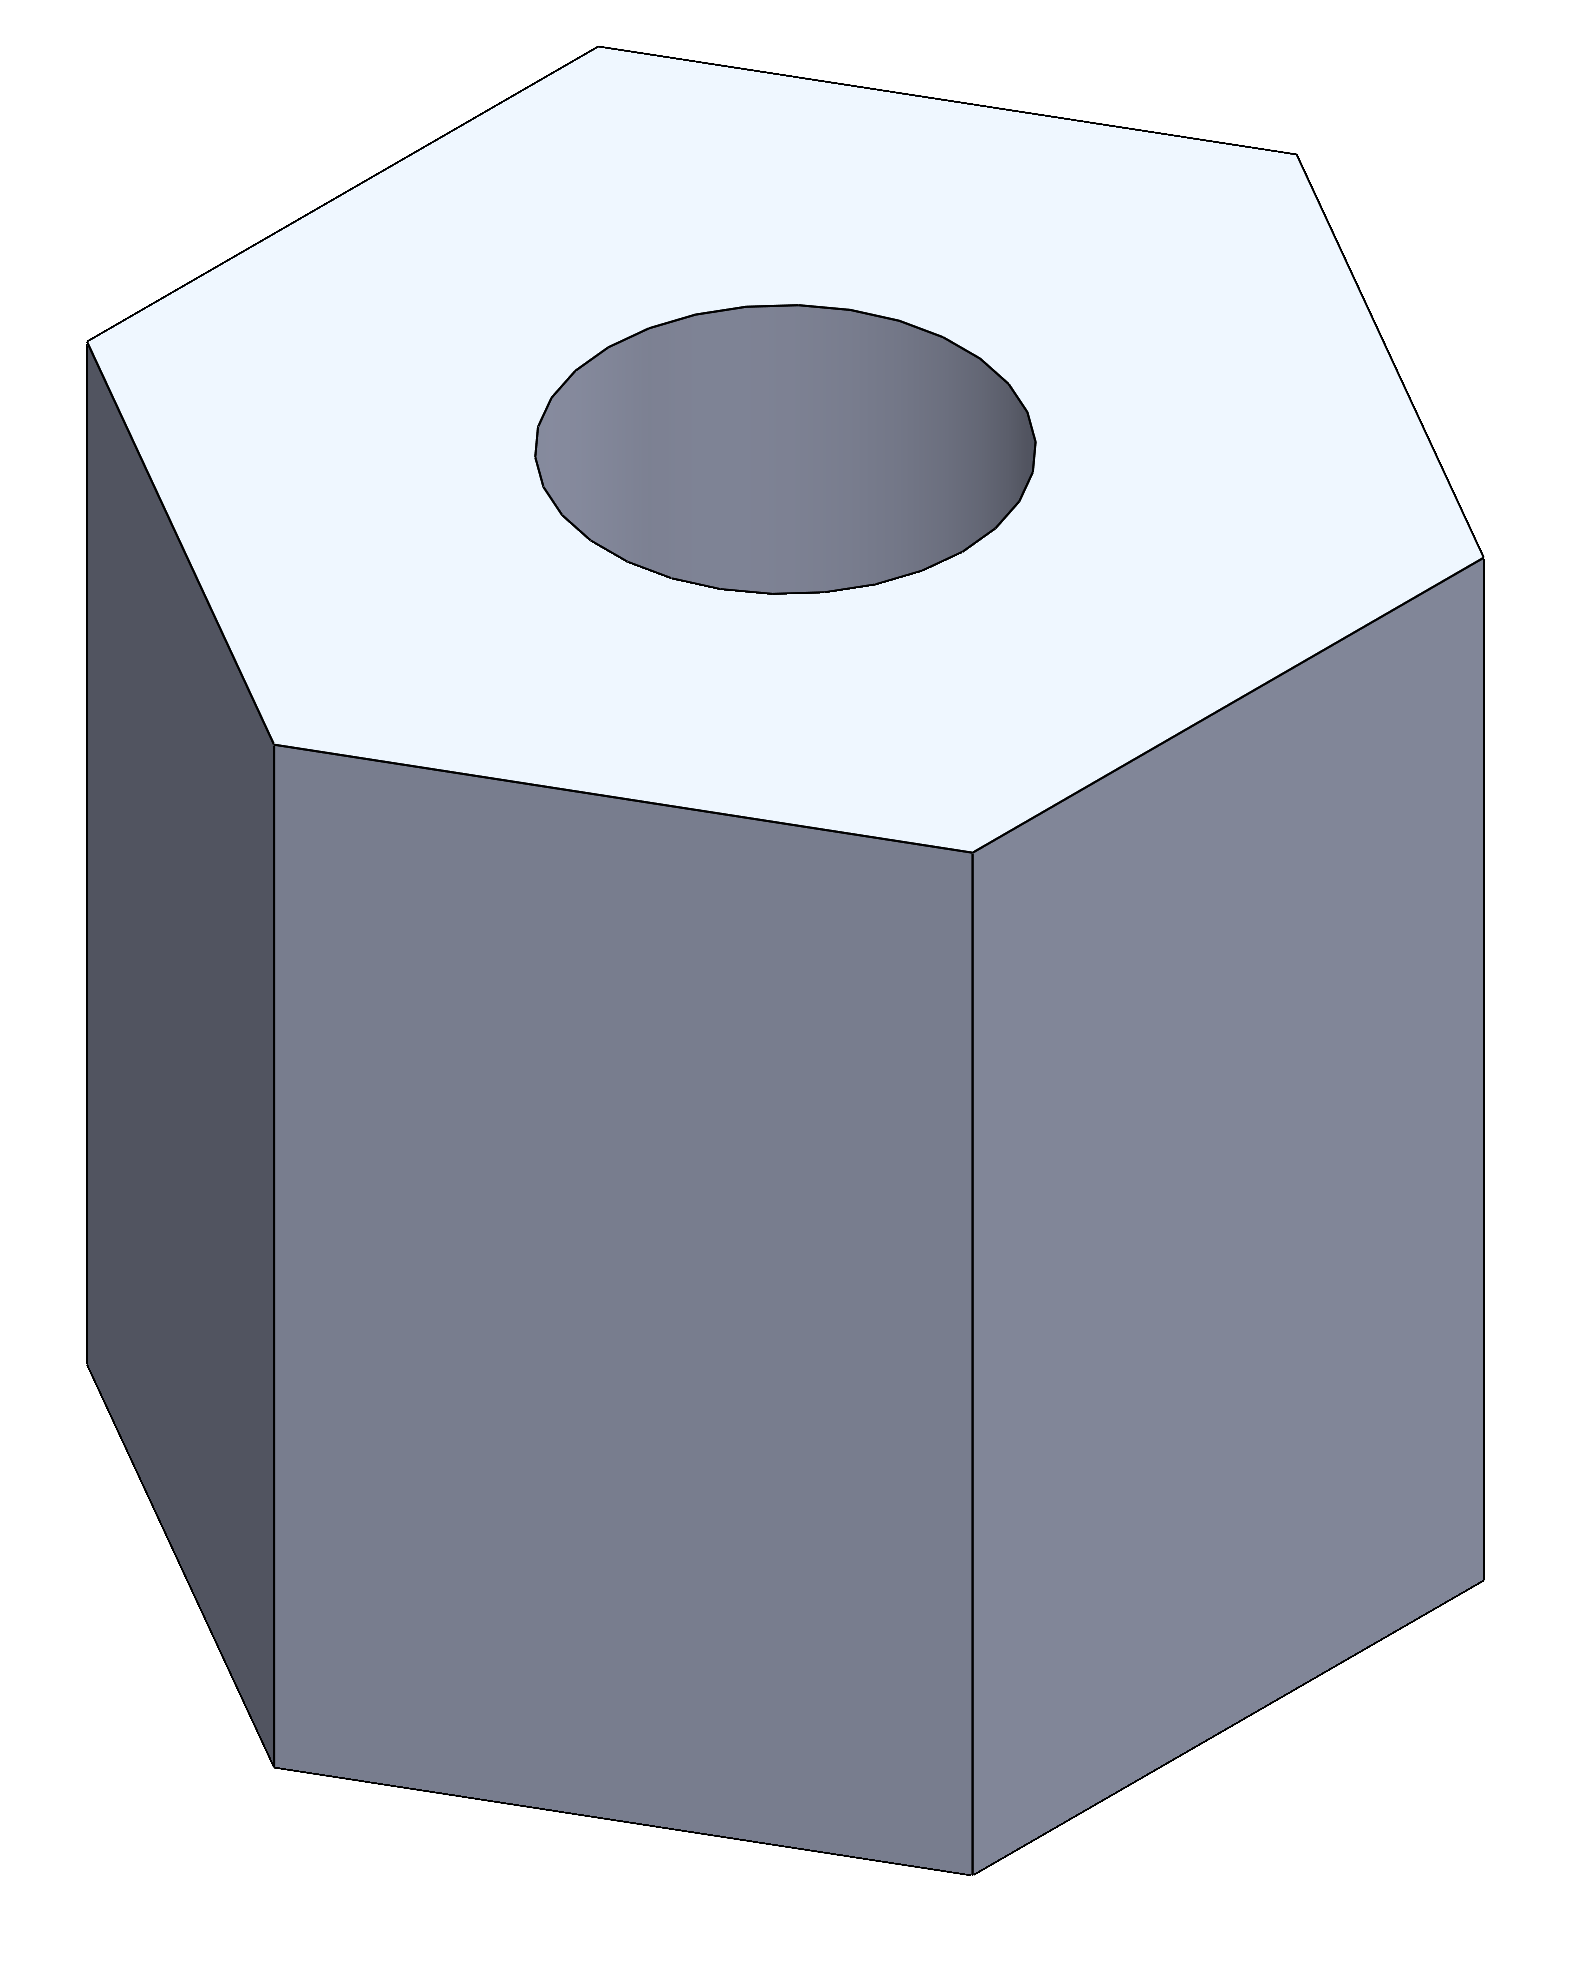
\includegraphics[width=\linewidth]{figures/parts/nut.PNG}
        \scriptsize Nut
      \end{minipage} &
      \begin{minipage}{0.3\linewidth}
        \centering
        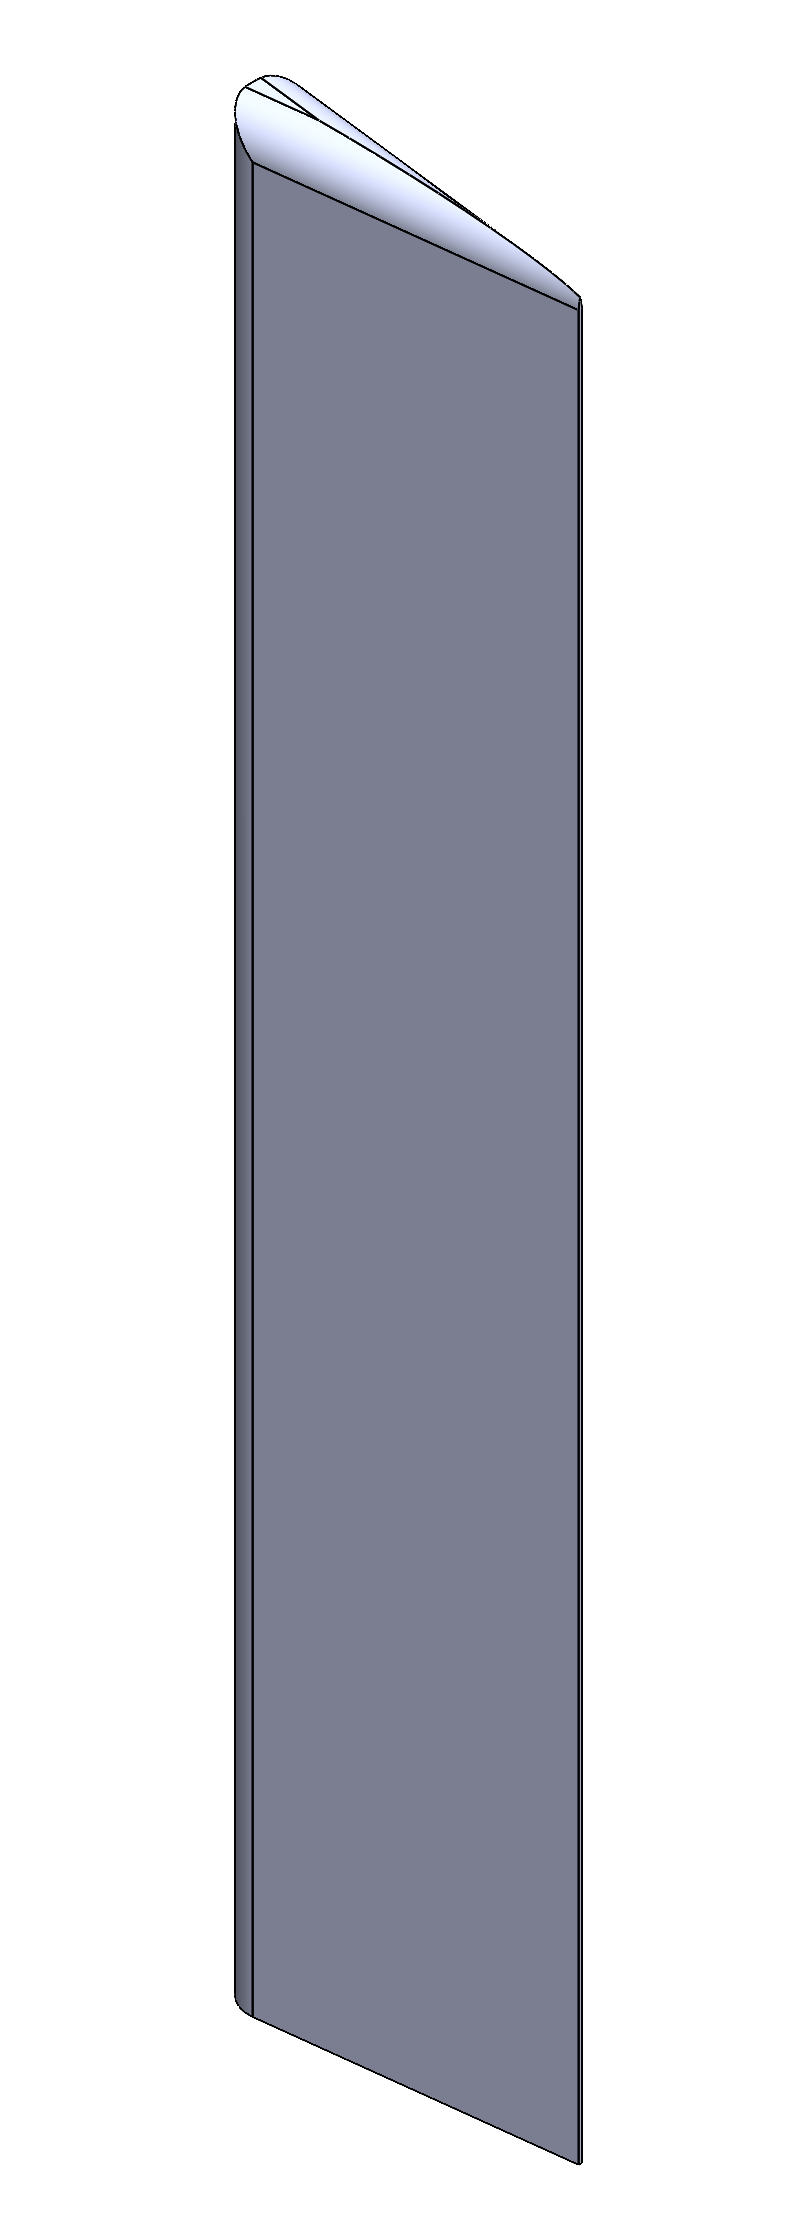
\includegraphics[width=\linewidth]{figures/parts/wedge.PNG}
        \scriptsize Wedge
      \end{minipage} &
      % Last column left blank
      \begin{minipage}{0.3\linewidth} \end{minipage} \\
    \end{tabular}
  \end{minipage}

  \caption{Shapes used in the dataset for MLP training.}
  \label{fig:part_shapes_grid}
\end{figure}














\subsection{Implementation Details}

The neural network model employed is a Multi-Layer Perceptron (MLP) designed to predict the quality of point clouds based on their extracted features. The architecture comprises an input layer, four hidden layers, and an output layer. Specifically, the hidden layers contain 64, 128, 128, and 64 units, respectively, and employ the ReLU activation function to introduce non-linearity. The output layer consists of a single unit that produces the final prediction value.

The model is implemented using the FLAX NNX framework, which is part of the JAX ecosystem. This enables efficient automatic differentiation and GPU acceleration, significantly reducing training times. The network is trained using the Adam optimizer, with a learning rate of 0.001 and a large batch size of 200{,}000. Training is performed for 1{,}000 epochs, and the loss function used is the mean squared error (MSE) between the predicted values and the ground truth labels.

Prior to being fed into the model, all features are standardized to improve convergence and generalization. The dataset is split into 80\% for training and 20\% for validation, ensuring that the model is evaluated on unseen data and can generalize effectively.

\begin{table}[htbp]
\centering
\begin{tabular}{|l|c|c|}
\hline
\textbf{Score} & \textbf{Dataset 1} & \textbf{Dataset 2} \\
\hline
R\textsuperscript{2} & 0.9818 & 0.9910 \\
MAE & 0.0425 & 0.0318 \\
MSE & 0.0137 & 0.0068 \\
RMSE & 0.1170 & 0.0825 \\
Max error & 1.8672 & 1.6806 \\
\hline
\end{tabular}
\vspace{0.5em}  % Adjust as needed
\caption{Comparison of model evaluation metrics between models trained on different datasets.}
\label{tab:model_metrics}
\end{table}

It is of interest to examine whether the model's predictions of surface density rely too heavily on a small subset of features. This is evaluated by analyzing which features are most influential and their relative importance in determining accurate predictions.

\begin{figure}[htbp]
\centering
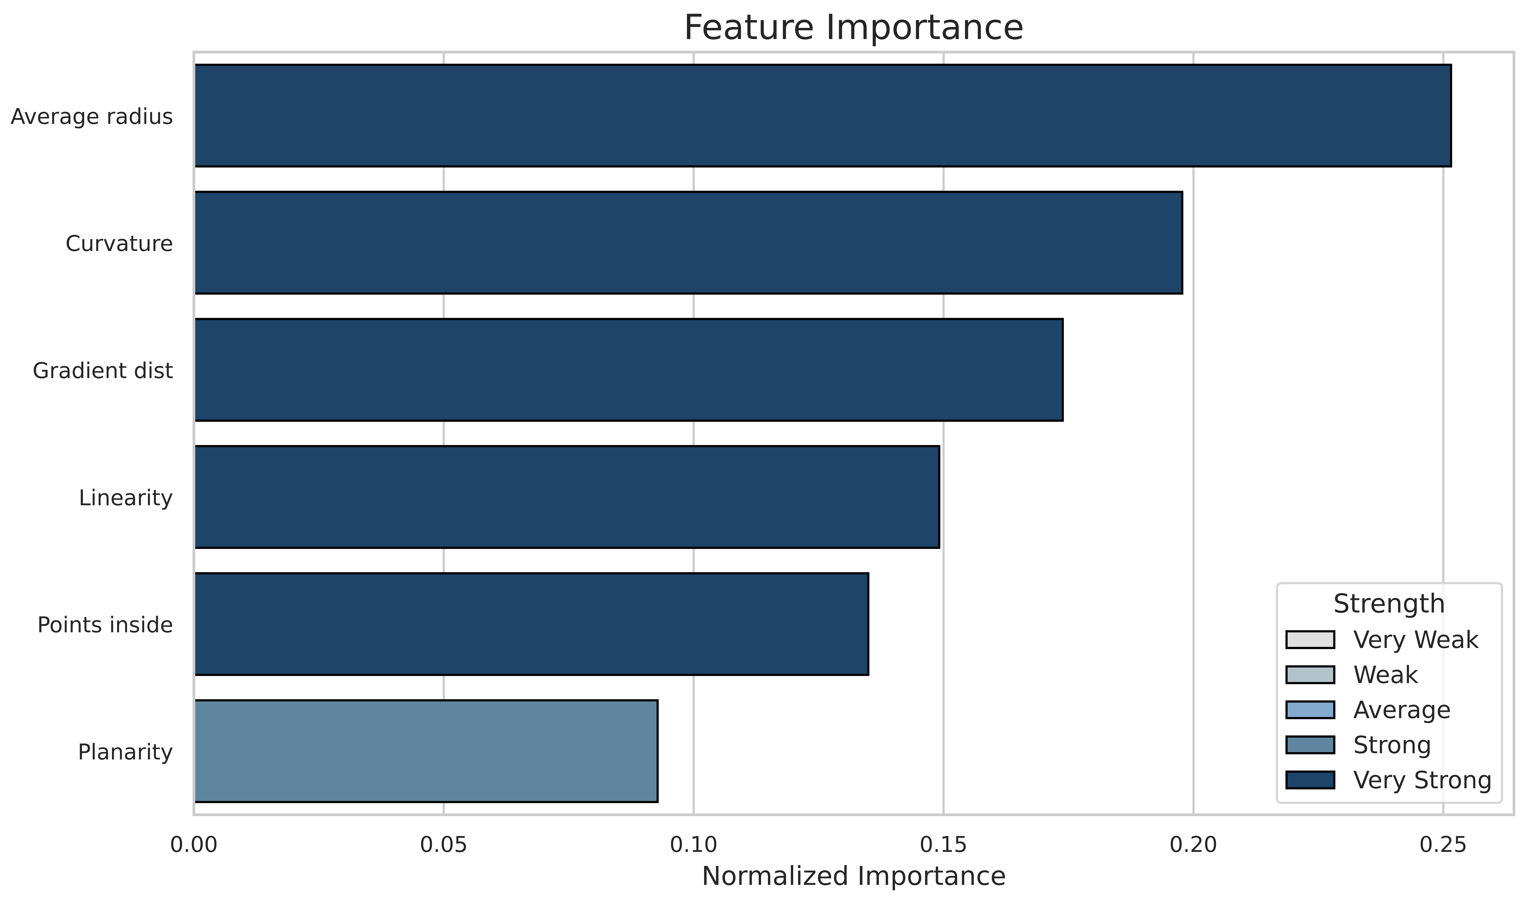
\includegraphics[width=0.5\textwidth]{figures/feature_importance_lowQ.png}
\caption{Visualization of the features used for training and their relative importance in the final model.}
\label{fig:feature_importance}
\end{figure}

A good distribution of importance between features show that the model use all features and not relying too much on a small number of features, see Figure(\ref{fig:feature_importance}).

While there is not a big difference in standard evaluation metrics between models trained on the two different datasets (Table \ref{tab:model_metrics}), there is a big difference the predictions of the models, especially in the lower end of mesh sizes. Therefore we need more evaluation criteria than the standard evaluation metrics.


\subsection{Evaluation Critaria}
\subsection{Results}

Other methods for calculating local PCQA exist [REF-Leihui], however this is a very time consuming method. Since this method utilize a neural network to predict the surface density/quality the predictions are instant, so the time consuming process of this method lies in the extraction of features. This process is done without looping but for a whole pointcloud in one go and the time it takes is related to how many points exist in the pointcloud. To determine the time taken for feature extraction, a pointcloud was created on the Ball (figure \ref{fig:part_shapes_grid}), but where the ball was varying in size, resulting in different pointcloud sizes. Figure \ref{fig:time} shows the time consumption of extracting features on these pointclouds.

\begin{figure}[htbp]
    \centering
    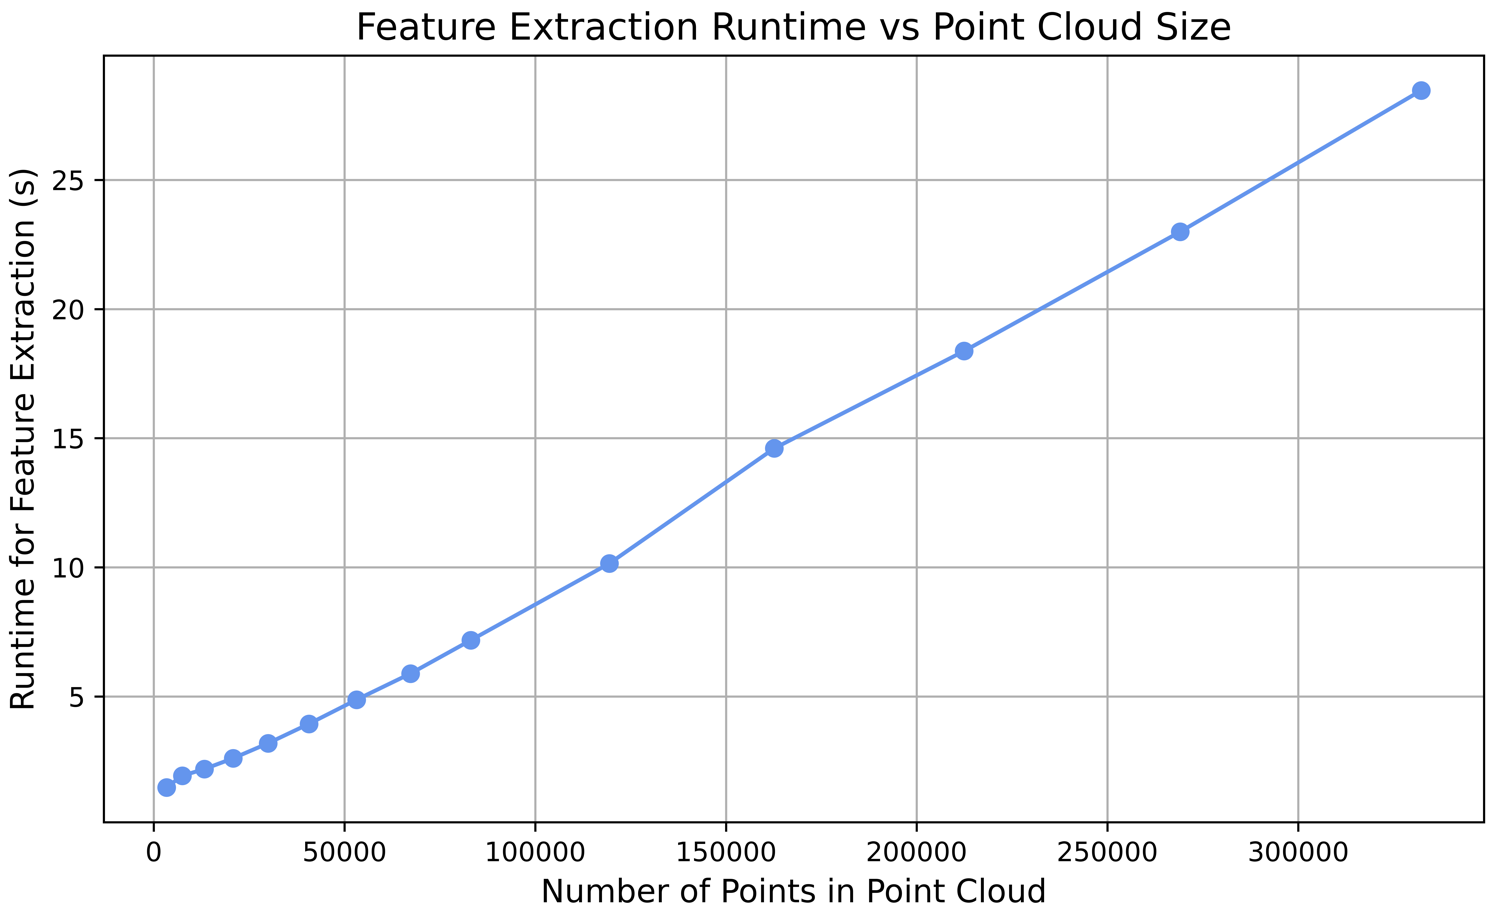
\includegraphics[width=0.5\textwidth]{figures/time_lowQ.png}
    \caption{Feature extraction time consumption for different pointcloud sizes.}
    \label{fig:time}
\end{figure}

To test the models trained on the two different datasets, the chainwheel was used to generate pointclouds in different mesh sizes to determine the robustness of the models. For the model trained on dataset 1, the predictions are very accurate for a mesh size of 0.5mm and again from meshsizes from 1mm to 2mm. However, mesh sizes between 0.6mm and 1mm gives some wrong predictions so the mean values are much lower than the actual label and the standard deviation is also large, see figure \ref{fig:pred_vs_label_first}.\\
The model trained on dataset 2 is much more robust, showing good predictions for all mesh sizes from 0.5mm to 2mm, with a very low standard deviation, see figure \ref{fig:pred_vs_label_better}. The variation in predictions also follow the tendency of surface density variation for the different mesh sizes as it naturally does as seen in figure \ref{fig:sd_mesh}. Here the variation of surface density is largest at smaller mesh sizes, and decrease as the mesh size goes up.

\begin{figure}[H]
    \centering
    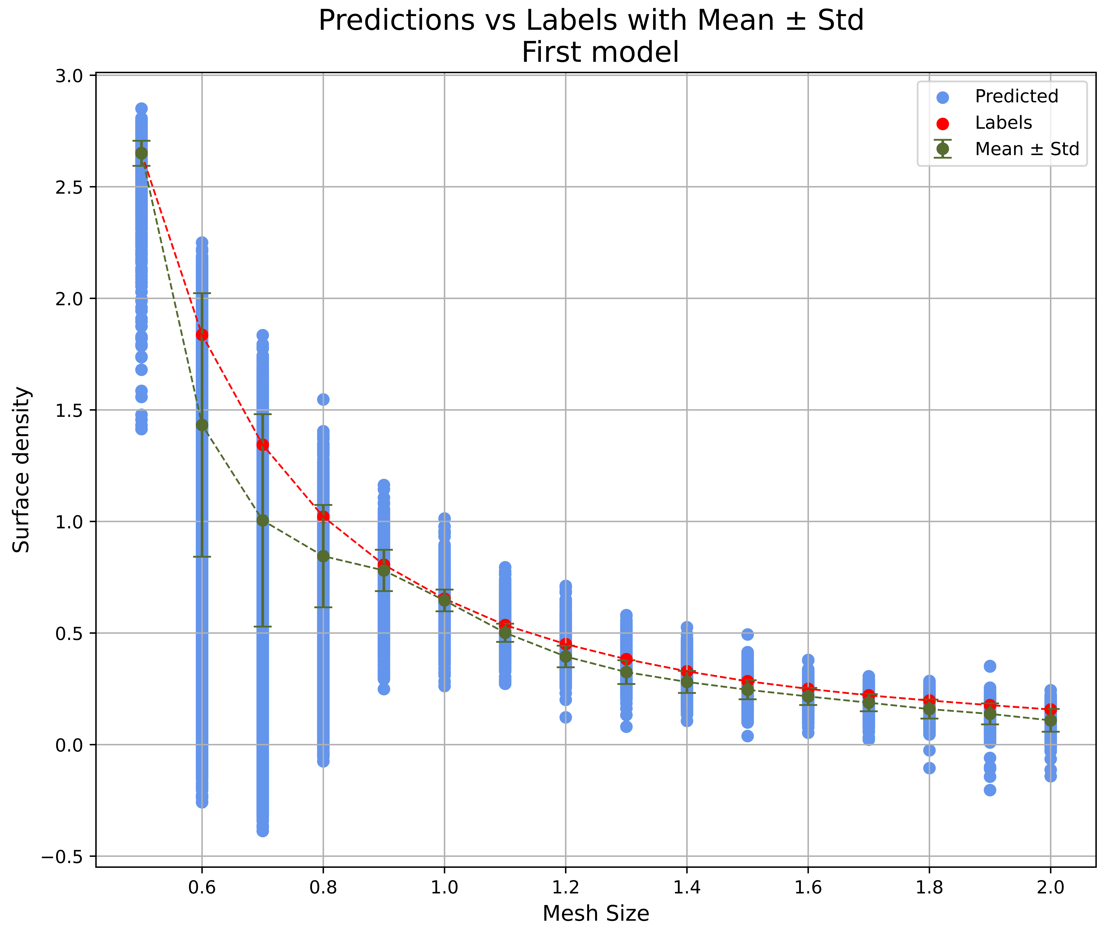
\includegraphics[width=0.5\textwidth]{figures/predict_vs_label_first_lowQ.png}
    \caption{Predicted surface densities vs truth label. Model trained on 0.5, 1.0 and 2.0 mm mesh sizes}
    \label{fig:pred_vs_label_first}
\end{figure}

\begin{figure}[H]
    \centering
    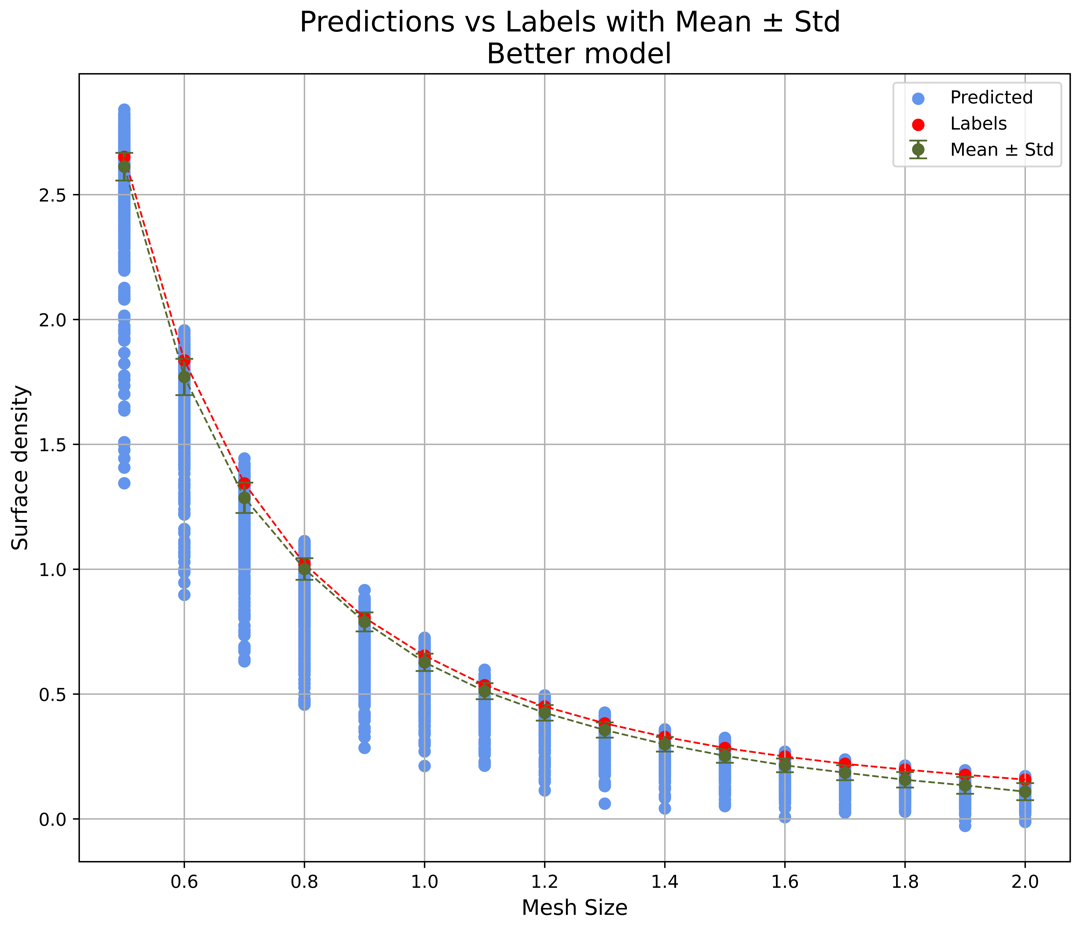
\includegraphics[width=0.5\textwidth]{figures/predict_vs_label_better_lowQ.png}
    \caption{Predicted surface densities vs truth label. Model trained on 0.5 to 2.0 mm mesh sizes with 0.1 mm intervals}
    \label{fig:pred_vs_label_better}
\end{figure}

The model should also mark areas where the mesh is incomplete, which simulate missing points that could stem from a incomplete scan of a part. To simulate bad scans holes of different sizes are made in the chain wheel pointcloud and then the quality is predicted. The predictions on these pointclouds shows that the holes are all marked as very low density areas, essentially marking areas where the pointcloud is incomplete, see figure \ref{fig:holes_predict}. The model finds holes as small as 5 points. The model also differentiates between holes that are present in the part and holes that are just from missing points, since the hole that goes through the chain wheel is left as a high density area.

\begin{figure*}[t]
    \centering
    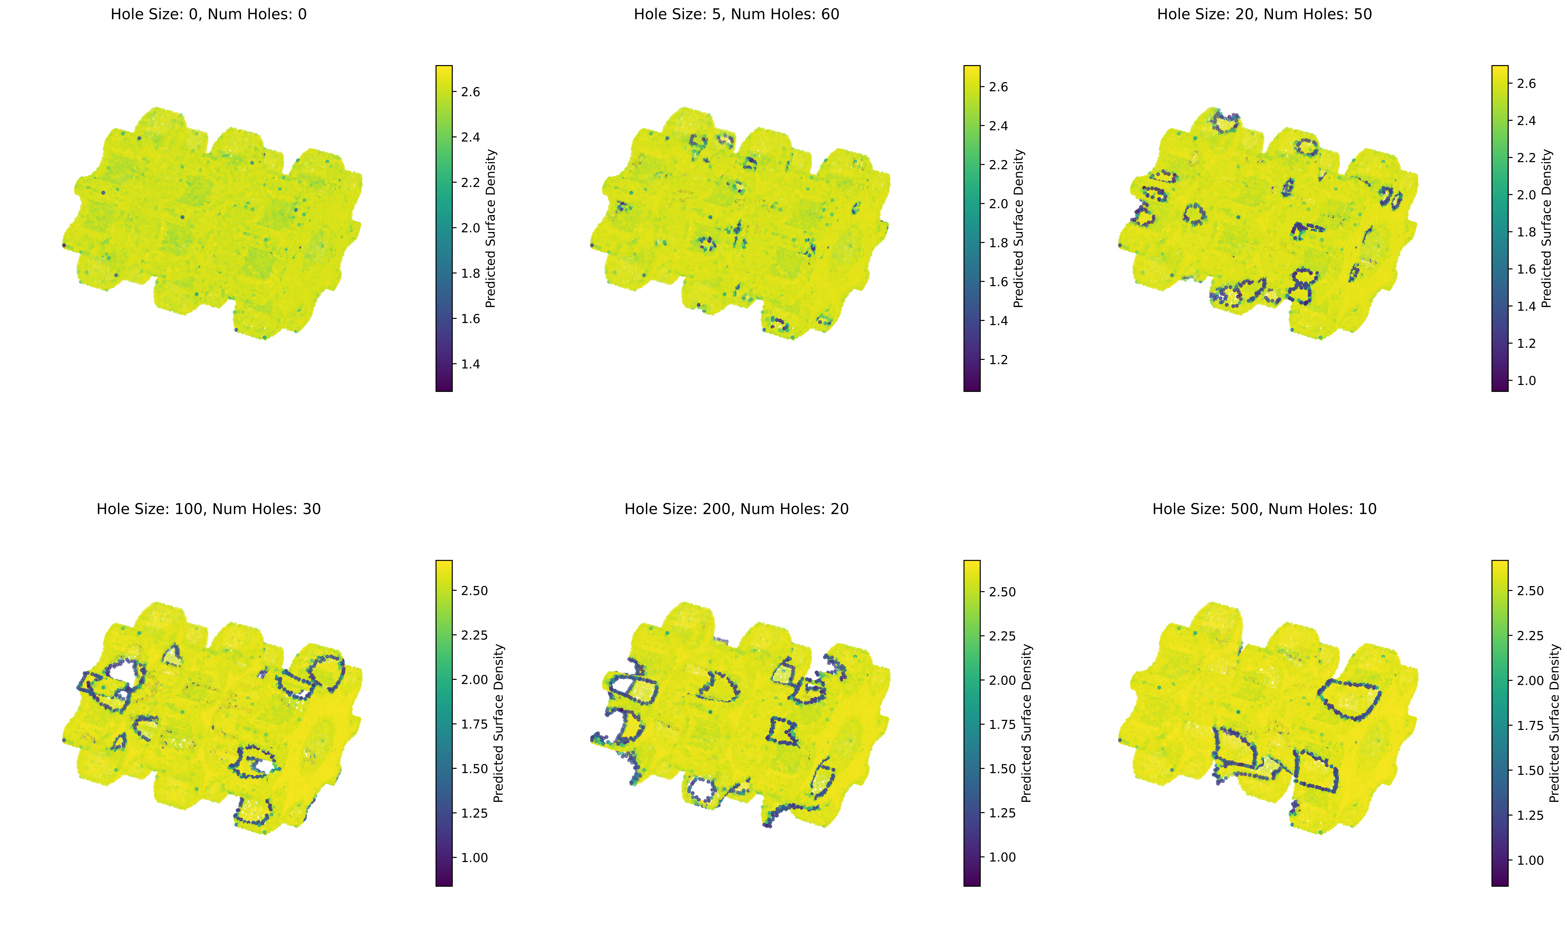
\includegraphics[width=\textwidth]{figures/result3_lowQ.png}
    \caption{Surface density predictions for the same pointcloud with varying hole sizes.}
    \label{fig:holes_predict}
\end{figure*}

The model also excels at predicting the correct surface density on the same part if they vary. This can be seen in figure \ref{fig:diff_mesh_predict}, where the chain-wheel was split up and meshed in different mesh sizes, but the whole pointcloud fed into the model as one pointcloud. Here it is seen that the model is consistent with prediction the correct corresponding surface density.


\begin{figure}[H]
    \centering
    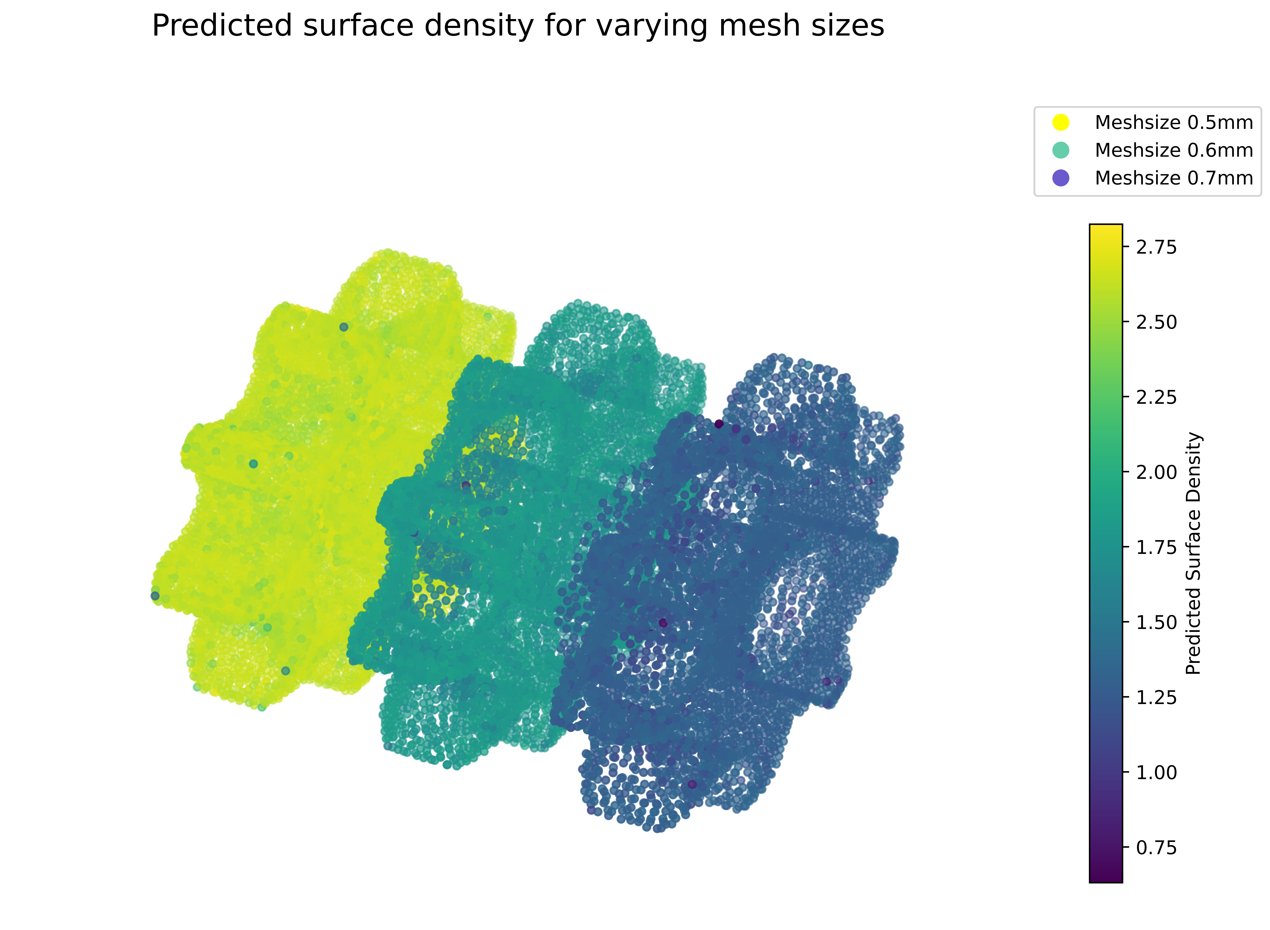
\includegraphics[width=0.5\textwidth]{figures/varying_meshsize_lowQ.png}
    \caption{Surface density predictions for mesh sizes: 0.5, 0.6 and 0.7}
    \label{fig:diff_mesh_predict}
\end{figure}


\section{Discussion and Future Works}
The model showed promising results, however there is some room for improvement. The improvements we think are most logical as the next step are presentedin this section, ranked after importance:

\begin{enumerate}
  \item \textbf{Improve accuracy of labels for imperfect data}
  \item \textbf{More diverse training data}
  \item \textbf{}
\end{enumerate}

\section{Conclusion}

\end{document}